% MSc thesis based on the PoliMi School of Industrial and Information
% Engineering template. Build from this directory with: latexmk -pdf Thesis.tex
\documentclass{Configuration_Files/PoliMi3i_thesis}

\usepackage{parskip}
\usepackage{setspace}
\usepackage{emptypage}
\usepackage{multicol}
\setlength\columnsep{15pt}
\setlength\parindent{10pt}
\raggedbottom

\usepackage{titlesec}
\titlespacing{\section}{0pt}{3.3ex}{2ex}
\titlespacing{\subsection}{0pt}{3.3ex}{1.65ex}
\titlespacing{\subsubsection}{0pt}{3.3ex}{1ex}

\usepackage[english]{babel}
\usepackage[utf8]{inputenc}
\usepackage[T1]{fontenc}
\usepackage[11pt]{moresize}
\usepackage{microtype}

\usepackage{graphicx}
\usepackage{svg}
\usepackage{transparent}
\usepackage{eso-pic}
\usepackage[export]{adjustbox}
\usepackage{tikz}
\usetikzlibrary{arrows.meta,positioning,shapes.geometric,fit,backgrounds}
\graphicspath{{./Images/}{../ILP/}{../results/serving_nixl_20260911_async_random500/}{../results/serving_nixl_20260911_async_random500_profile/}}
\usepackage{caption}
\usepackage{subcaption}
\usepackage{xcolor}
\usepackage{amsthm,thmtools}
\usepackage{float}

\usepackage{amsmath}
\usepackage{amssymb}
\usepackage{amsfonts}
\usepackage{bm}
\usepackage[overload]{empheq}
\usepackage{fix-cm}

\usepackage{tabularx}
\usepackage{longtable}
\usepackage{colortbl}
\usepackage{booktabs}
\usepackage{multirow}

\usepackage{listings}
\newfloat{algorithm}{tbp}{loa}[chapter]
\floatname{algorithm}{Algorithm}
\lstdefinestyle{code}{
  basicstyle=\ttfamily\footnotesize,
  breaklines=true,
  frame=single,
  columns=fullflexible,
  keepspaces=true,
  showstringspaces=false
}

\usepackage[colorlinks=true,linkcolor=black,anchorcolor=black,citecolor=black,
  filecolor=black,menucolor=black,runcolor=black,urlcolor=bluepoli]{hyperref}
\hypersetup{
  pdftitle={Contention-Aware Expert Migration for Dynamic Load Balancing in
    Mixture-of-Experts Serving},
  pdfauthor={WU CAO},
  pdfsubject={Master's thesis in High Performance Computing Engineering},
  pdfkeywords={mixture of experts, expert parallelism, EPLB, expert migration,
    network contention, vLLM, NIXL}
}
\usepackage{cleveref}
\usepackage[square,numbers,sort&compress]{natbib}
\bibliographystyle{abbrvnat}

\usepackage{pdfpages}
\usepackage{afterpage}
\usepackage{fancyhdr}
\usepackage{fancyvrb}
\usepackage[acronym,nomain]{glossaries}
\usepackage{enumitem}
\fancyhf{}

% Define blue color typical of polimi
\definecolor{bluepoli}{cmyk}{0.4,0.1,0,0.4}
\definecolor{Green}{RGB}{30, 170, 0}

% Custom theorem environments
\declaretheoremstyle[
  headfont=\color{bluepoli}\normalfont\bfseries,
  bodyfont=\color{black}\normalfont\itshape,
]{colored}

% Set-up caption colors
%\captionsetup[figure]{labelfont={color=bluepoli}} % Set colour of the captions
%\captionsetup[table]{labelfont={color=bluepoli}} % Set colour of the captions
%\captionsetup[algorithm]{labelfont={color=bluepoli}} % Set colour of the captions
\captionsetup{font=bf}

\theoremstyle{colored}
\newtheorem{theorem}{Theorem}[chapter]
\newtheorem{proposition}{Proposition}[chapter]
\newtheorem{definition}{Definition}[chapter]

% Enhances the features of the standard "table" and "tabular" environments.
\newcommand\T{\rule{0pt}{2.6ex}}
\newcommand\B{\rule[-1.2ex]{0pt}{0pt}}

% Pseudo-code algorithm descriptions.
\newcounter{algsubstate}
\renewcommand{\thealgsubstate}{\alph{algsubstate}}
\newenvironment{algsubstates}
  {\setcounter{algsubstate}{0}%
   \renewcommand{\STATE}{%
     \stepcounter{algsubstate}%
     \Statex {\small\thealgsubstate:}\space}}
  {}

% New font size
\newcommand\numfontsize{\@setfontsize\Huge{200}{60}}

% Title format: chapter
\titleformat{\chapter}[hang]{
\fontsize{50}{20}\selectfont\bfseries\filright}{\textcolor{bluepoli} \thechapter\hsp\hspace{2mm}\textcolor{bluepoli}{|   }\hsp}{0pt}{\huge\bfseries \textcolor{bluepoli}
}

% Title format: section
\titleformat{\section}
{\normalfont\Large\bfseries}
{\thesection.}{1em}{}
%{\color{bluepoli}\normalfont\Large\bfseries}
%{\color{bluepoli}\thesection.}{1em}{}

% Title format: subsection
\titleformat{\subsection}
{\normalfont\large\bfseries}
{\thesubsection.}{1em}{}
%{\color{bluepoli}\normalfont\large\bfseries}
%{\color{bluepoli}\thesubsection.}{1em}{}

% Title format: subsubsection
\titleformat{\subsubsection}
{\normalfont\bfseries}
{\thesubsubsection.}{1em}{}
%{\color{bluepoli}\normalfont\large\bfseries}
%{\color{bluepoli}\thesubsubsection.}{1em}{}

% Shortening for setting no horizontal-spacing
\newcommand{\hsp}{\hspace{0pt}}

\makeatletter
% Renewcommand: cleardoublepage including the background pic
\renewcommand*\cleardoublepage{%
  \clearpage\if@twoside\ifodd\c@page\else
  \null
  \AddToShipoutPicture*{\BackgroundPic}
  \thispagestyle{empty}%
  \newpage
  \if@twocolumn\hbox{}\newpage\fi\fi\fi}
\makeatother

%For correctly numbering algorithms
\numberwithin{algorithm}{chapter}

\newcommand{\code}[1]{\texttt{#1}}
\newcommand{\SI}[2]{#1\,#2}
\newcommand{\system}{contention-aware migration batching}
\newcommand{\prnumber}{\#52641}

\makeglossaries

\newacronym{e2e}{E2E}{end-to-end}
\newacronym{ecmp}{ECMP}{equal-cost multi-path}
\newacronym{ep}{EP}{expert parallelism}
\newacronym{eplb}{EPLB}{Expert Parallel Load Balancing}
\newacronym{gpu}{GPU}{graphics processing unit}
\newacronym{ilp}{ILP}{integer linear program}
\newacronym{llm}{LLM}{large language model}
\newacronym{moe}{MoE}{Mixture of Experts}
\newacronym{nic}{NIC}{network interface controller}
\newacronym{nixl}{NIXL}{NVIDIA Inference Xfer Library}
\newacronym{nvtx}{NVTX}{NVIDIA Tools Extension}
\newacronym{rdma}{RDMA}{remote direct memory access}
\newacronym{tpot}{TPOT}{time per output token}
\newacronym{ttft}{TTFT}{time to first token}
\newacronym{ucx}{UCX}{Unified Communication X}


\begin{document}

\fancypagestyle{plain}{%
  \fancyhf{}
  \fancyhead[RO,RE]{\thepage}
  \renewcommand{\headrulewidth}{0pt}
  \renewcommand{\footrulewidth}{0pt}}

\pagestyle{empty}
\frontmatter

\puttitle{
  title=Contention-Aware Expert Migration for Dynamic Load Balancing in Mixture-of-Experts Serving,
  name=WU CAO,
  course=High Performance Computing Engineering \\ Ingegneria del Calcolo ad Alte Prestazioni,
  ID=11036000,
  advisor=Prof. Massimo Tornatore,
  coadvisor={Assistant Prof. Qiaolun Zhang},
  academicyear={2026--2027},
}

\startpreamble
\setcounter{page}{1}

\chapter*{Abstract}
Mixture-of-Experts (MoE) language models increase parameter capacity while
activating only a subset of experts for each token. At inference time, expert
parallelism distributes those experts across accelerators. The resulting load
is input dependent: a small group of experts can become disproportionately
popular, leaving some ranks overloaded while others are underutilized. Expert
Parallel Load Balancing (EPLB) addresses this imbalance by periodically
changing expert placement and migrating expert weights. In asynchronous EPLB,
inference continues during migration; consequently, migration traffic and
latency-sensitive inference traffic share the same network resources.

This thesis studies the network interference created when many point-to-point
expert migrations are submitted simultaneously. It first formulates migration
scheduling as an integer linear program (ILP) that minimizes the worst modeled
inference time under link contention, subject to a hard rank-disjoint-flow
constraint. The formulation exposes the central
trade-off: spreading transfers over several batches reduces peak link load but
can lengthen the migration itself. Based on this insight, a lightweight online
scheduler is designed for vLLM. Expert transfers are represented as a rank
communication multigraph, coalesced by directed rank pair, and greedily grouped
into batches in which every rank participates in at most one directed flow.
Schedules for all MoE layers are prepared once per rebalance cycle, while
weight transfer and activation remain layer by layer. The implementation is opt-in, applies
only to asynchronous EPLB, preserves the original synchronous path, and was
merged upstream in vLLM pull request \prnumber.

The system is evaluated on four nodes connected by \SI{10}{Gb/s} Ethernet,
each with one Quadro RTX 6000 GPU, using Qwen3-30B-A3B-Instruct-2507, Ray,
and the NIXL communication backend. In a controlled 500-request A/B benchmark,
batching increased output throughput by 2.28\%, reduced median and P99
time-per-output-token by 1.94\% and 0.87\%, and reduced median and P99
end-to-end latency by 3.18\% and 1.50\%. P99 aggregate NIC traffic on the head
node decreased by 10.24\%. NVTX-only Nsight Systems traces measured 34
cycle-wide scheduler invocations per rank; the largest cumulative scheduling
cost was \SI{302.081}{ms}, equal to 0.285\% of the \SI{105.932}{s} serving-time
reduction observed in the independent A/B run. These measurements show that,
for the evaluated configuration, conservative rank-disjoint batching can trade
a small amount of CPU scheduling work and migration serialization for lower
network bursts and improved serving performance.

\textbf{Keywords:} mixture of experts, expert parallelism, load balancing,
expert migration, network contention, vLLM, NIXL

\chapter*{Abstract in lingua italiana}
I modelli linguistici Mixture-of-Experts (MoE) aumentano la capacità in termini
di parametri attivando, per ciascun token, solo un sottoinsieme degli esperti.
Durante l'inferenza, l'expert parallelism distribuisce tali esperti tra più
acceleratori. Il carico risultante dipende dall'input: alcuni esperti possono
diventare molto più richiesti di altri, sovraccaricando determinati rank e
lasciandone altri sottoutilizzati. L'Expert Parallel Load Balancing (EPLB)
riduce questo squilibrio modificando periodicamente il posizionamento degli
esperti e migrandone i pesi. Nella modalità asincrona, l'inferenza continua
durante la migrazione; il traffico di migrazione e quello dell'inferenza
condividono quindi le stesse risorse di rete.

Questa tesi analizza l'interferenza di rete causata dall'invio simultaneo di
molte migrazioni punto-punto. Il problema viene inizialmente formulato come un
programma lineare intero (ILP), con l'obiettivo di minimizzare il peggior tempo
di inferenza modellato in presenza di contesa sui link. La formulazione mette
in evidenza il compromesso fondamentale: distribuire i trasferimenti su più
batch riduce il picco di traffico, ma può aumentare la durata complessiva della
migrazione. Sulla base di questa osservazione è stato progettato uno scheduler
online leggero per vLLM. I trasferimenti sono rappresentati come un multigrafo
di comunicazione tra rank, aggregati per coppia diretta e raggruppati con un
algoritmo greedy in batch nei quali ogni rank partecipa al massimo a un flusso
diretto.
Gli schedule di tutti i layer MoE sono calcolati una sola volta per ciclo di
riequilibrio, mentre il trasferimento e l'attivazione restano sequenziali per
layer. L'implementazione è opzionale, riguarda esclusivamente EPLB asincrono e
mantiene invariato il percorso sincrono; è stata integrata upstream in vLLM
tramite la pull request \prnumber.

La valutazione usa quattro nodi connessi tramite Ethernet a \SI{10}{Gb/s},
ciascuno dotato di una GPU Quadro RTX 6000, con il modello
Qwen3-30B-A3B-Instruct-2507, Ray e il backend NIXL. In un benchmark A/B
controllato di 500 richieste, il batching aumenta il throughput di output del
2.28\%, riduce il tempo per token di output P50/P99 dell'1.94\%/0.87\% e la
latenza end-to-end P50/P99 del 3.18\%/1.50\%. Il P99 del traffico NIC aggregato
sul nodo principale diminuisce del 10.24\%. Le tracce NVTX raccolte con Nsight
Systems misurano 34 invocazioni dello scheduler per rank; il costo cumulativo
massimo è \SI{302.081}{ms}, pari allo 0.285\% dei \SI{105.932}{s} risparmiati
nel benchmark A/B indipendente. Per la configurazione studiata, i risultati
mostrano che un batching conservativo e privo di conflitti tra rank può ridurre
i picchi di rete e migliorare le prestazioni di serving con un costo CPU
contenuto.

\textbf{Parole chiave:} mixture of experts, expert parallelism, bilanciamento
del carico, migrazione degli esperti, contesa di rete, vLLM, NIXL

\thispagestyle{empty}
\tableofcontents
\thispagestyle{empty}
\cleardoublepage

\addtocontents{toc}{\vspace{2em}}
\mainmatter

\chapter{Introduction}
\section{Motivation}

Large language model serving is a systems problem as much as a model problem.
An online service must keep expensive accelerators occupied, admit requests
with different prompt and generation lengths, manage a dynamically growing
key--value cache, and coordinate communication across devices. vLLM addresses
several of these concerns through continuous batching and PagedAttention
\cite{kwon2023vllm}. The adoption of sparse \gls{moe} models introduces a
further challenge: the compute and communication performed for a token depend
on which experts the router selects.

An MoE layer contains many feed-forward expert networks but activates only a
small subset for each token. This conditional computation increases model
capacity without making the arithmetic cost proportional to the total number
of parameters \cite{shazeer2017moe,fedus2021switch}. It also makes the runtime
load data dependent. Tokens in a batch do not necessarily select experts
uniformly, and the popularity distribution can shift as the request mix
changes. When experts are sharded across devices with \gls{ep}, an overloaded
expert becomes an overloaded rank. Faster ranks then wait at collective
communication boundaries, so one local imbalance can reduce cluster-wide
throughput.

\gls{eplb} mitigates this problem by observing expert usage and periodically
computing a new physical placement. Popular experts can be replicated and the
mapping between logical experts and physical slots can be changed. Applying a
new placement, however, requires copying expert weights between ranks. These
objects are much larger than control messages and the transfers use the same
host and network resources as foreground inference. This thesis focuses on a
specific but consequential phase of EPLB: scheduling those expert migrations.

The original execution path posts the point-to-point operations for a layer as
one group. This minimizes the number of explicit communication rounds, which
is attractive if migration completion time is the only objective. During
asynchronous EPLB, however, inference does not stop. A rank that simultaneously
sends to and receives from several peers can create a short traffic burst at
its network interface. The burst may compete with token dispatch, result
collection, tensor-parallel communication, or other inference-related traffic.
Thus, the schedule that completes migration soonest is not necessarily the
schedule that gives users the best latency while migration is in progress.

The distinction is especially important in a multi-node deployment whose
network is slower than local accelerator memory. Expert migration is a
background maintenance operation; the foreground objective is serving quality.
The central hypothesis of this work is therefore:

\begin{quote}
Limiting the number of simultaneous migration peers per rank can reduce network
bursts enough to improve foreground serving, even when doing so introduces
additional migration rounds.
\end{quote}

\section{Research questions}

The thesis is organized around four research questions.

\begin{enumerate}[label=\textbf{RQ\arabic*:},leftmargin=2.2cm]
  \item \textbf{How should expert migration contention be represented?}
  A useful model must distinguish expert count, source and destination ranks,
  network paths, and link capacities while remaining simple enough to explain
  the scheduler's behavior.

  \item \textbf{What scheduling rule is suitable for the online path?}
  An exact optimizer is valuable as a design tool, but a production scheduler
  must be deterministic, fast, dependency-light, and compatible with the
  existing replicated placement maps.

  \item \textbf{Can the implementation preserve EPLB semantics?}
  Batching must move every required expert exactly once, retain local-copy and
  replica semantics, respect the communicator lifecycle, and leave the legacy
  path unchanged unless the feature is explicitly enabled.

  \item \textbf{Does reduced migration contention improve serving?}
  The answer requires both user-visible metrics and direct network evidence.
  Throughput, \gls{ttft}, \gls{tpot}, and end-to-end latency are measured
  together with one-second NIC byte counters and scheduler profiling.
\end{enumerate}

\section{Contributions}

This work makes the following contributions.

\begin{itemize}
  \item It separates two objectives that can otherwise be conflated: minimizing
  migration completion time and minimizing the interference experienced by
  concurrent inference.

  \item It formulates contention-aware migration scheduling as an \gls{ilp}.
  The model assigns coalesced directed rank-pair flows to batches, constrains
  each rank to one incident flow per batch, estimates routed link load, and
  minimizes the worst modeled inference time. This is an exact optimum only
  within the hard rank-disjoint-flow policy and the stated linear model. An illustrative
  eight-rank topology exposes the trade-off rather than claiming a calibrated
  latency predictor or proving that rank-disjoint scheduling is universally best.

  \item It designs a production-oriented greedy scheduler. The problem is
  reduced to deterministic first-fit edge coloring of a communication graph.
  Multiple experts with the same directed source--destination pair are
  coalesced, independent rank pairs can progress concurrently, and every rank
  participates in at most one directed flow in a batch.

  \item It integrates the scheduler into asynchronous vLLM EPLB. Scheduling
  for all 48 MoE layers is invoked once per rebalance cycle, while transfers
  remain layer by layer. The feature is opt-in and synchronous EPLB retains the
  original path because inference is already paused in that mode.

  \item It evaluates the complete serving system and profiles the scheduler.
  The final contribution was reviewed and merged into upstream vLLM as pull
  request \prnumber\ \cite{vllmpr52641}.
\end{itemize}

\section{Scope and claims}

The evaluation is deliberately narrow enough to be reproducible. It uses one
four-node cluster, one model, one communication backend, one workload shape,
and one A/B run per condition. This supports a case study and an engineering
validation, not a universal performance claim. The experiment establishes
that the proposed mechanism works and is beneficial under the measured
configuration. It does not establish how the effect scales to modern
datacenter GPUs, RDMA fabrics, different expert sizes, or more ranks.

The thesis also distinguishes artifacts by purpose. The ILP is an offline
analytical baseline. The greedy algorithm is the deployed scheduler. Older
experiments created during design iteration are not used for the final result;
all reported E2E values come from one archived A/B directory, and all scheduler
costs come from a separate archived profiling directory. This provenance is
specified in \cref{ch:methodology} and the appendices.

\section{Thesis structure}

\Cref{ch:background} introduces sparse MoE inference, expert parallelism,
vLLM EPLB, and asynchronous migration. \Cref{ch:related-work} reviews MoE
communication, coflow scheduling, and graph-based migration grouping.
\Cref{ch:formulation,ch:design} then develop the contention model and the
production scheduler within one proposed-system chapter.
\Cref{ch:methodology,ch:results} document the evaluation procedure and report
the E2E, NIC, and profiling results within one experimental-evaluation chapter.
Finally, \cref{ch:conclusions} summarizes the findings, limitations, and future
work.


\chapter{Background and Related Work}
\label{ch:background}

\section{Autoregressive language-model serving}

An autoregressive language model generates one token at a time. Serving a
request normally has two computational phases. During \emph{prefill}, the
model processes the prompt and constructs the key--value cache. During
\emph{decode}, the service repeatedly executes the model to produce one or a
small number of new tokens. Prefill has substantial parallel work over prompt
tokens, whereas decode is iterative and often sensitive to memory access,
scheduling delay, and interference.

Modern serving engines batch requests whose sequences are at different
positions. vLLM introduced PagedAttention to reduce fragmentation and enable
flexible sharing of KV-cache blocks, thereby increasing the number of requests
that can be served concurrently \cite{kwon2023vllm}. Continuous batching makes
resource utilization higher, but also means that a background operation may
affect multiple requests in different phases at the same time.

Four metrics are central in this thesis. Output throughput is the number of
generated tokens per second over the measured interval. \gls{ttft} is the time
from request submission until its first output token, so it includes admission,
queueing, and prefill. \gls{tpot} averages the gaps between output tokens after
the first token and is primarily associated with decode. End-to-end latency
measures the complete request. Reporting both median and P99 values separates
typical behavior from tail behavior. Precise definitions are given in
\cref{app:metrics}.

\section{Sparse mixture-of-experts models}

The sparsely gated MoE layer was developed as a practical form of conditional
computation \cite{shazeer2017moe}. Let $x$ denote a token representation,
$E_i$ the $i$th expert, and $g_i(x)$ a router weight. A simplified MoE output is

\begin{equation}
  y(x)=\sum_{i\in\operatorname{TopK}(g(x))} g_i(x) E_i(x).
\end{equation}

Only the selected experts execute for $x$. This decouples total parameter
capacity from active arithmetic. GShard demonstrated large-scale conditional
computation with automatic sharding \cite{lepikhin2020gshard}; Switch
Transformer simplified routing to one expert per token and highlighted both
the scaling opportunity and the communication and load-balancing challenges
\cite{fedus2021switch}. Recent open models continue this direction. Qwen3
includes dense and MoE variants \cite{yang2025qwen3}, while DeepSeek-V3 uses a
large sparse architecture and an auxiliary-loss-free training-time balancing
strategy \cite{deepseek2024v3}.

The evaluated Qwen3-30B-A3B-Instruct-2507 checkpoint has 30.5 billion total
parameters, approximately 3.3 billion activated parameters, 48 layers, 128
experts, and eight selected experts per token \cite{qwen3modelcard}. The gap
between total and active parameters makes it a useful serving model: compute
is sparse, but expert weights remain substantial objects that must be placed
and occasionally copied.

\section{Expert parallelism}

In \gls{ep}, experts are distributed across ranks. A token is dispatched to
the ranks holding its selected experts; expert outputs are then returned to
the rank that continues the model computation. EP avoids replicating every
expert on every device, but introduces all-to-all-style communication and a
dependence on balanced rank workloads.

Let $a_{l,e}$ be the number of token assignments to logical expert $e$ in layer
$l$ over an observation window. If rank $r$ hosts a set $H_{l,r}$, a simple
load estimate is

\begin{equation}
  L_{l,r}=\sum_{e\in H_{l,r}} a_{l,e}.
\end{equation}

Even if training encourages globally balanced routing, a finite serving window
can be skewed. Request language, task, domain, and generation state can all
change which experts are selected. Moreover, the system cares about load per
physical rank, not only load per logical expert. Several moderately popular
experts placed together can overload a rank.

\section{Expert Parallel Load Balancing in vLLM}

vLLM's EPLB records expert usage over a configurable window and periodically
computes a new placement. Redundant experts add physical slots beyond the
number required for one copy of each logical expert. The balancer can use those
slots to replicate hot experts and distribute their assignments. vLLM exposes
the observation window, rebalance interval, redundancy, asynchronous mode,
policy, and migration communicator through \code{EPLBConfig}
\cite{vllmeplbdocs}.

Placement is represented by replicated logical-to-physical and
physical-to-logical mappings for every MoE layer. Once a new map is available,
each rank can independently derive which logical experts it loses, keeps, or
gains. Local rearrangements copy weights between slots on the same rank.
Remote gains require a source rank that already owns the logical expert and a
point-to-point weight transfer.

Synchronous and asynchronous EPLB have different performance objectives. A
synchronous rearrangement pauses inference. In that setting, extra sequential
communication rounds directly extend the pause, so quickly completing the
migration is the natural goal. Asynchronous EPLB moves experts in a background
worker while inference continues. It transfers one layer and coordinates its
activation with forward progress before proceeding. Here, the migration has
more time, but interference with foreground work matters. This thesis changes
only the asynchronous path and retains the synchronous behavior.

\begin{figure}[t]
  \centering
  \begin{tikzpicture}[
    node distance=13mm and 11mm,
    box/.style={draw,rounded corners,align=center,minimum width=31mm,minimum height=10mm},
    arr/.style={-{Latex[length=2mm]},thick}
  ]
    \node[box] (metrics) {Per-layer expert\\usage window};
    \node[box,right=of metrics] (placement) {EPLB policy\\new placement};
    \node[box,right=of placement] (schedule) {Migration\\schedule};
    \node[box,below=of schedule] (transfer) {Background layer\\transfer};
    \node[box,left=of transfer] (activate) {Mapping swap at\\safe boundary};
    \node[box,left=of activate] (serve) {Foreground\\inference};
    \draw[arr] (metrics) -- (placement);
    \draw[arr] (placement) -- (schedule);
    \draw[arr] (schedule) -- (transfer);
    \draw[arr] (transfer) -- (activate);
    \draw[arr] (activate) -- (serve);
    \draw[arr] (serve) -- (metrics);
    \draw[arr,dashed]
      (serve.south) to[out=-65,in=-115]
      node[below]{shared network resources} (transfer.south);
  \end{tikzpicture}
  \caption{Simplified asynchronous EPLB control loop. The contribution of this
  thesis is the migration-scheduling block and its execution path.}
  \label{fig:eplb-loop}
\end{figure}

\section{NIXL communication}

\gls{nixl} provides a transfer abstraction for distributed inference across
heterogeneous memory and storage. A transfer agent manages registered memory,
remote metadata, backend selection, and asynchronous point-to-point requests
\cite{nixlguide}. vLLM supports NIXL as an EPLB communicator and can also use
Gloo or other backends depending on mode and configuration
\cite{vllmconfigdocs}.

The final evaluation explicitly selects NIXL. This choice matters for both
performance and correctness. In the implementation evaluated here,
\code{execute()} drains the queued transfer operations and clears the transfer
context. Consequently, every migration batch must restore the layer context,
post only that batch's sends and receives, and call \code{execute()}. Moving
the call outside the loop would collapse the batch boundaries and defeat the
scheduler's concurrency constraint.


\chapter{Problem Formulation}
\label{ch:formulation}

\subsection{Migration instructions and flows}

Consider one MoE layer before and after a rebalance. Let $R$ be the set of EP
ranks and $E$ the set of logical experts. The old and new placement arrays
contain the expert identifier stored in every physical slot. Comparing the two
arrays determines which rank gains each expert. If a destination already owns
a copy, only a local rearrangement is needed; otherwise, one existing source
copy must supply the new replica.

A raw migration instruction is a tuple $(s,d,e)$ containing source rank $s$,
destination rank $d$, and logical expert $e$. Multiple experts may have the
same ordered rank pair. Since such transfers have identical endpoint
constraints, the scheduler coalesces them into a flow

\begin{equation}
  p=(s_p,d_p,E_p),
\end{equation}

where $E_p$ is the ordered set of expert identifiers assigned to the pair. Let
$w_p=|E_p|$ be the flow size in expert units. Coalescing reduces scheduler work
and prevents identical rank pairs from being artificially separated across
batches.

When an expert has several old replicas and several new destinations, the
source choice is also a scheduling decision in principle. The production
implementation preserves the existing vLLM assignment: destinations are
distributed as evenly as possible over source replicas in deterministic rank
order. Migration batching changes ordering, not placement semantics or replica
ownership.

\subsection{Network model}

The offline model supports an explicit network graph and a compact two-tier
topology. In the latter, GPUs connect to server endpoints through local links;
server endpoints share a slower inter-server network. Let $\mathcal{L}$ be the
set of routed links and $C_l>0$ the capacity of link $l$. Fixed shortest-path
ECMP determines $f_{p,l}$, the fraction of flow $p$ routed over $l$. In the
illustrative instance there is a single path for each flow, so $f_{p,l}$ is
binary.

The model measures flow size in expert units rather than bytes. It therefore
assumes equal expert payloads within the layer. This matches the evaluated
model architecture but would need extension for heterogeneous or quantized
experts. Following the bottleneck and residual-bandwidth view used in coflow
scheduling \cite{chowdhury2014varys}, it represents the bandwidth left by
foreground inference as $C_l(1-\rho)$, where $\rho\in[0,1)$ is the fraction of
link capacity occupied by inference. Varys estimates residual bandwidth from
measurements; the illustrative ILP instead uses one normalized $\rho$ for all
links. It is therefore a scenario parameter, not a deployment-independent
empirical constant.

\subsection{Constrained integer linear program}

Let $P$ be the set of coalesced flows and $B=\{0,\ldots,|P|-1\}$ a safe upper
bound on candidate batches. The binary assignment variable is

\begin{equation}
x_{p,b}=\begin{cases}
1 & \text{if flow $p$ is assigned to batch $b$},\\
0 & \text{otherwise.}
\end{cases}
\end{equation}

Binary variable $y_b$ indicates whether batch $b$ is active. Every flow is
assigned exactly once:

\begin{equation}
  \sum_{b\in B}x_{p,b}=1 \qquad \forall p\in P.
  \label{eq:flow-once}
\end{equation}

The conservative endpoint constraint permits at most one incident coalesced
directed flow for a rank in a batch:

\begin{equation}
  \sum_{p:s_p=r\,\lor\,d_p=r}x_{p,b}\leq 1
  \qquad \forall r\in R,\;\forall b\in B.
  \label{eq:endpoint}
\end{equation}

Assignments activate their batch, and symmetry is reduced by requiring active
batches to form a prefix:

\begin{align}
  x_{p,b} &\leq y_b,\\
  y_b &\geq y_{b+1}.
\end{align}

The migration load on routed link $l$ in batch $b$ is

\begin{equation}
  Q_{l,b}=\sum_{p\in P}w_p f_{p,l}x_{p,b}.
\end{equation}

Let $T_0$ be inference time without migration. The model assumes slowdown is
linear in migration load relative to residual link capacity:

\begin{equation}
  T_{\mathrm{infer}} \geq
  T_0\left(1+\frac{Q_{l,b}}{C_l(1-\rho)}\right)
  \qquad \forall l,b.
  \label{eq:slowdown}
\end{equation}

The maximum-over-links structure follows the standard bottleneck observation
that a collection of parallel network flows is limited by its most heavily
loaded endpoint or link \cite{chowdhury2014varys}. The endpoint limit is a
policy constraint rather than a conclusion produced by
the solver. The ILP therefore finds the best schedule among assignments under
the rank-disjoint-flow constraint; it does not compare that constraint with
higher degrees of migration concurrency. The primary optimization inside this
feasible region is

\begin{equation}
  \min T_{\mathrm{infer}},
\end{equation}

which is equivalent under this model to minimizing the maximum normalized link
load over all batches. After fixing the optimum value, a second solve minimizes
$\sum_b y_b$ as a tie-break. Batch count is not mixed into the primary
objective, avoiding an arbitrary weighted sum between foreground latency and
migration duration. The implementation uses SciPy's mixed-integer programming
interface backed by HiGHS \cite{scipy2020,huangfu2018highs}.

\subsection{Migration-time diagnostic}

The ILP deliberately optimizes modeled inference time, not migration time. To
make the trade-off visible, it reports a diagnostic. The duration of batch $b$
is approximated by its bottleneck-link service time:

\begin{equation}
  T_b=\max_{l\in\mathcal{L}}\frac{Q_{l,b}}{C_l}.
\end{equation}

Given a per-batch launch or synchronization overhead $\delta$, total migration
time is estimated as

\begin{equation}
  T_{\mathrm{migration}}=\sum_b T_b+\delta\sum_b y_b.
  \label{eq:migration-time}
\end{equation}

Splitting one busy batch into several lighter batches can reduce the maximum in
\cref{eq:slowdown} while increasing the sum in \cref{eq:migration-time}. This
is not a contradiction. The two quantities answer different questions: the
first represents foreground interference; the second represents how long the
background reconfiguration remains unfinished.

\subsection{Illustrative hotspot instance}

The example contains eight GPU ranks, two GPUs per server, local-link capacity
18, network-link capacity 2, and $\rho=0.6$, leaving 40\% normalized link
headroom for migration. Eight migrations create a shared-network hotspot. The
numeric units and the 40\% headroom are a deliberately stressed illustrative
scenario, not measurements from the experimental cluster. Because the same
$\rho$ multiplies every candidate link--batch pair, changing it uniformly
rescales the reported value of $T_{\mathrm{infer}}$ but does not change which
batch assignment minimizes the objective. A production predictor should
replace it with per-link residual bandwidth measured at runtime.

\begin{figure}[p]
  \centering
  \begin{subfigure}[t]{0.31\textwidth}
    \centering
    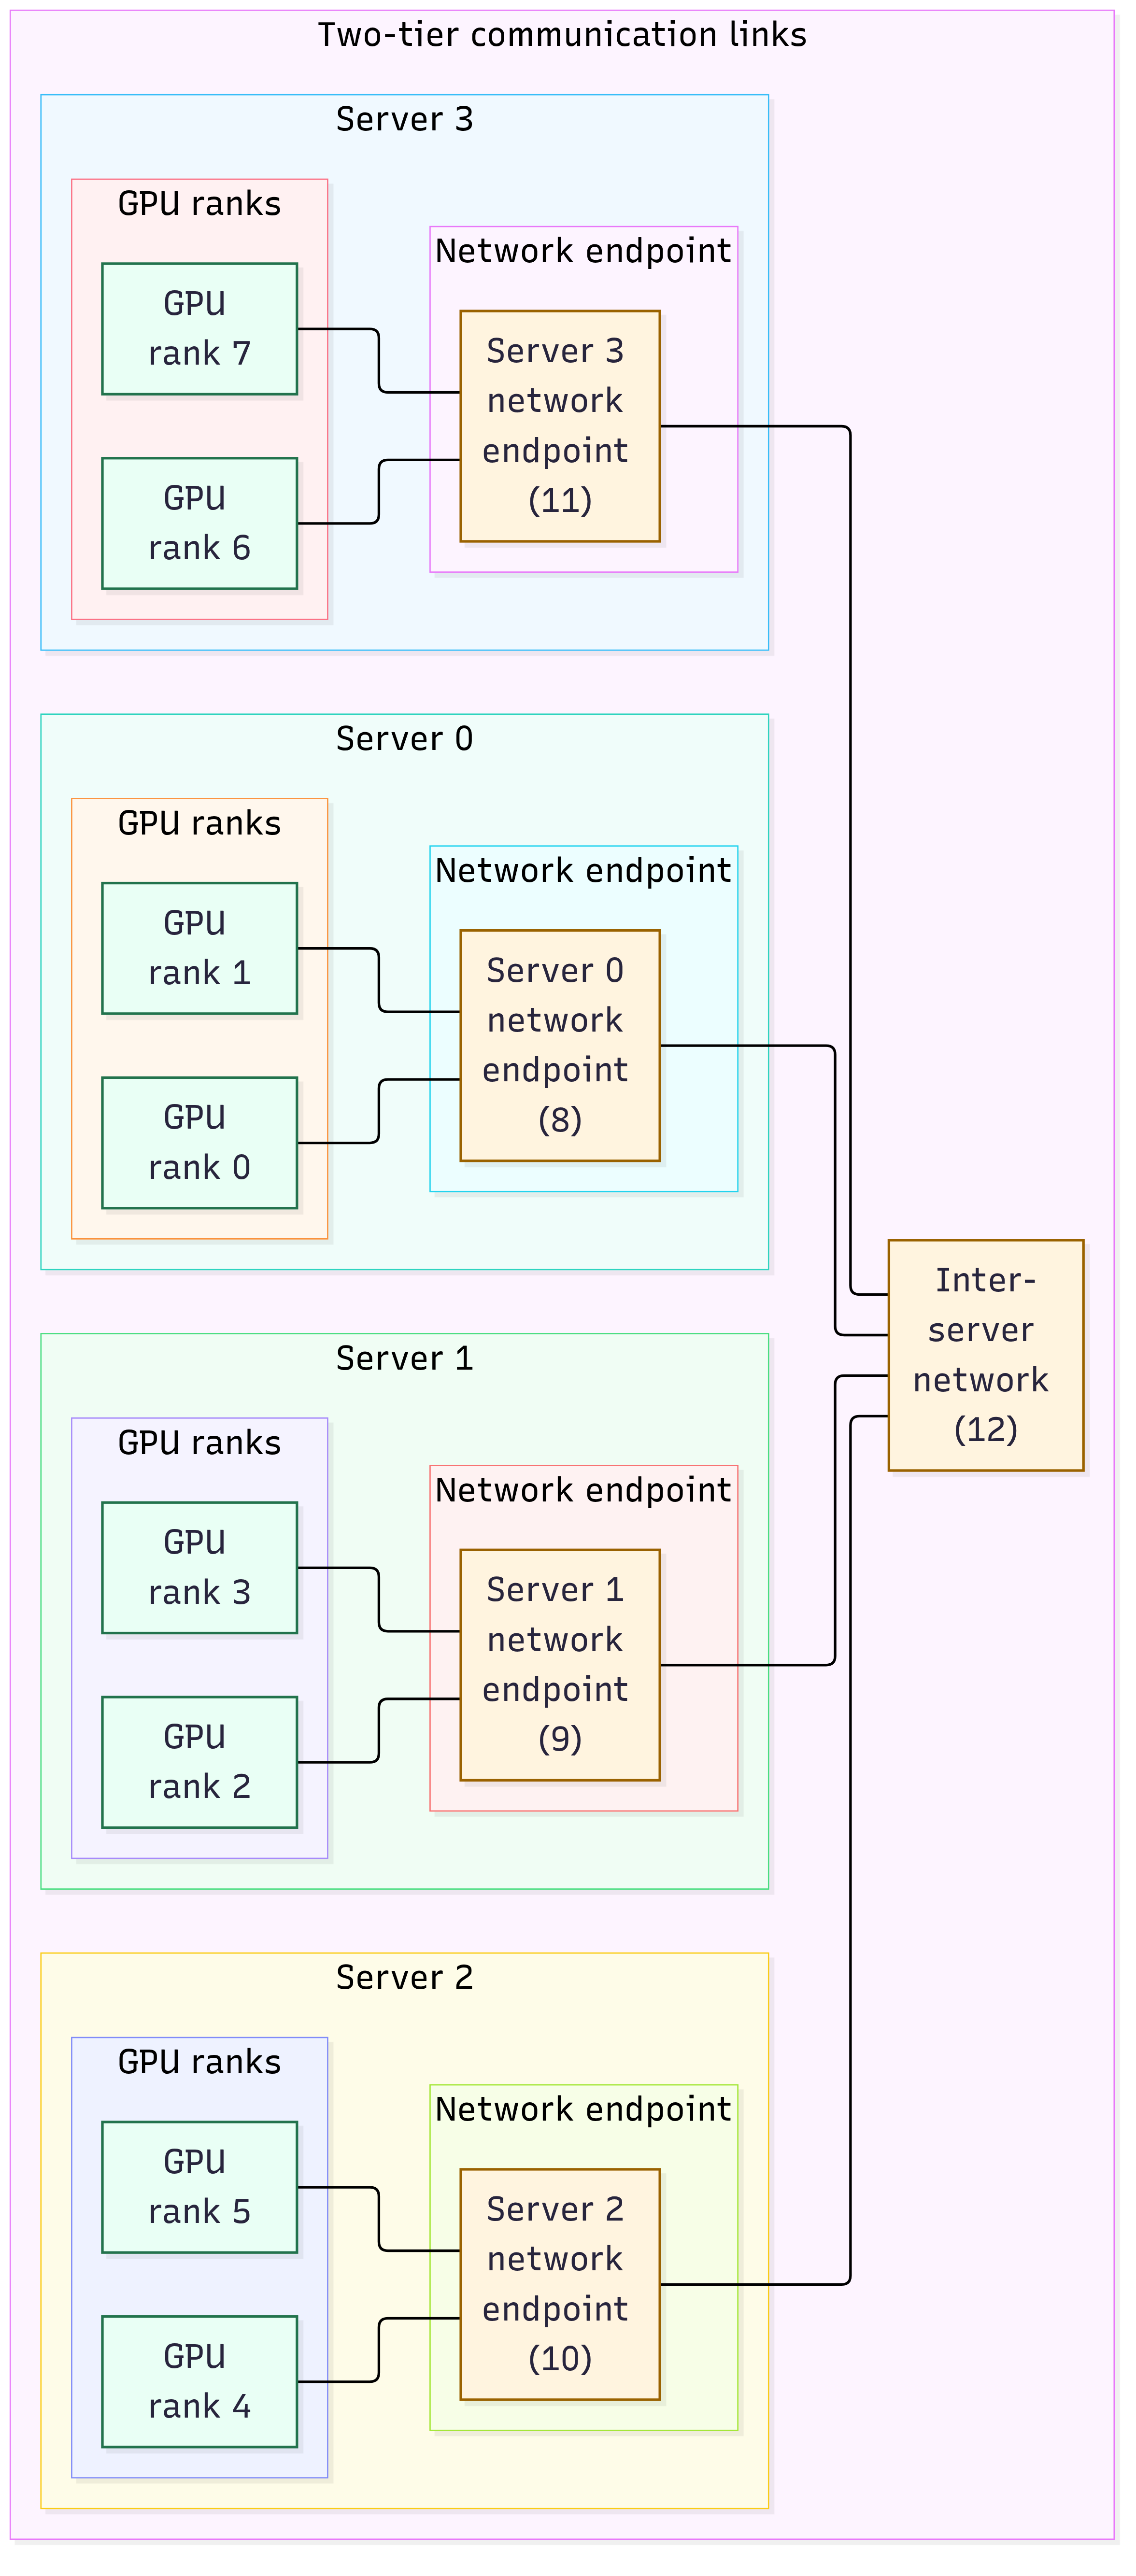
\includegraphics[width=\linewidth]{example_hotspot_links.png}
    \caption{Two-tier routed-link topology.}
  \end{subfigure}\hfill
  \begin{subfigure}[t]{0.31\textwidth}
    \centering
    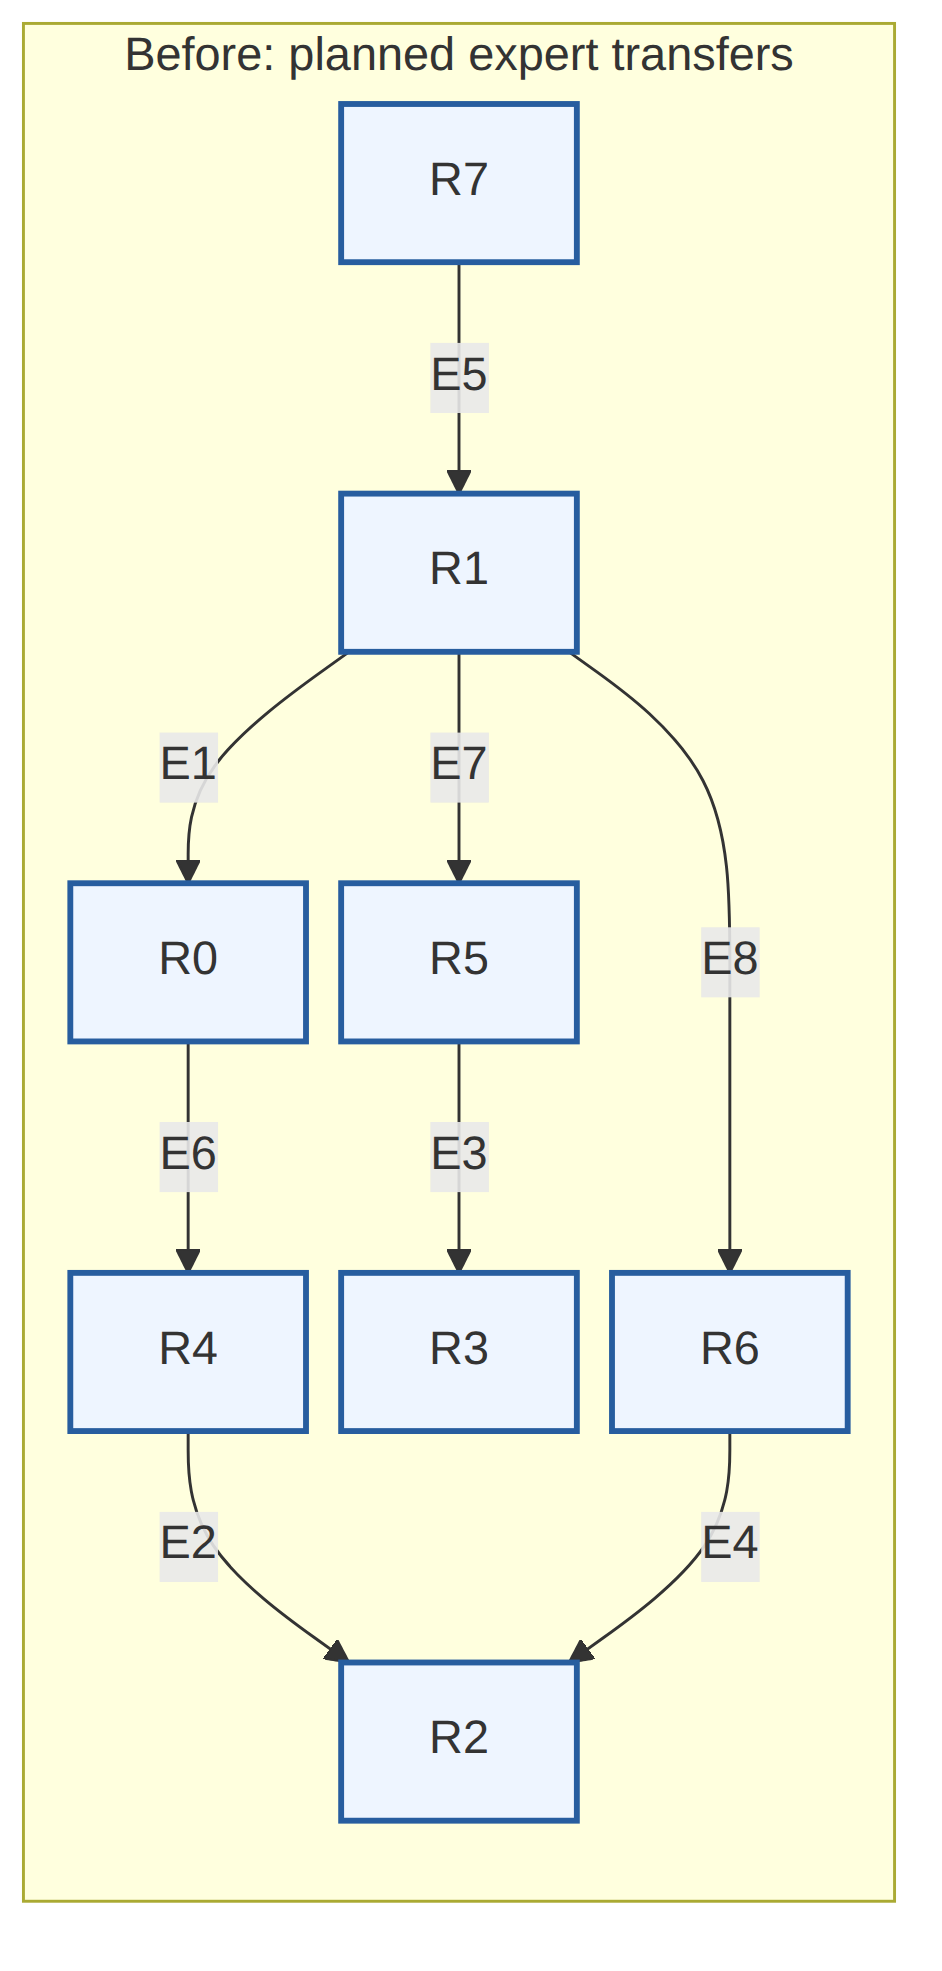
\includegraphics[width=\linewidth]{example_hotspot_before.png}
    \caption{All migrations issued together.}
  \end{subfigure}\hfill
  \begin{subfigure}[t]{0.31\textwidth}
    \centering
    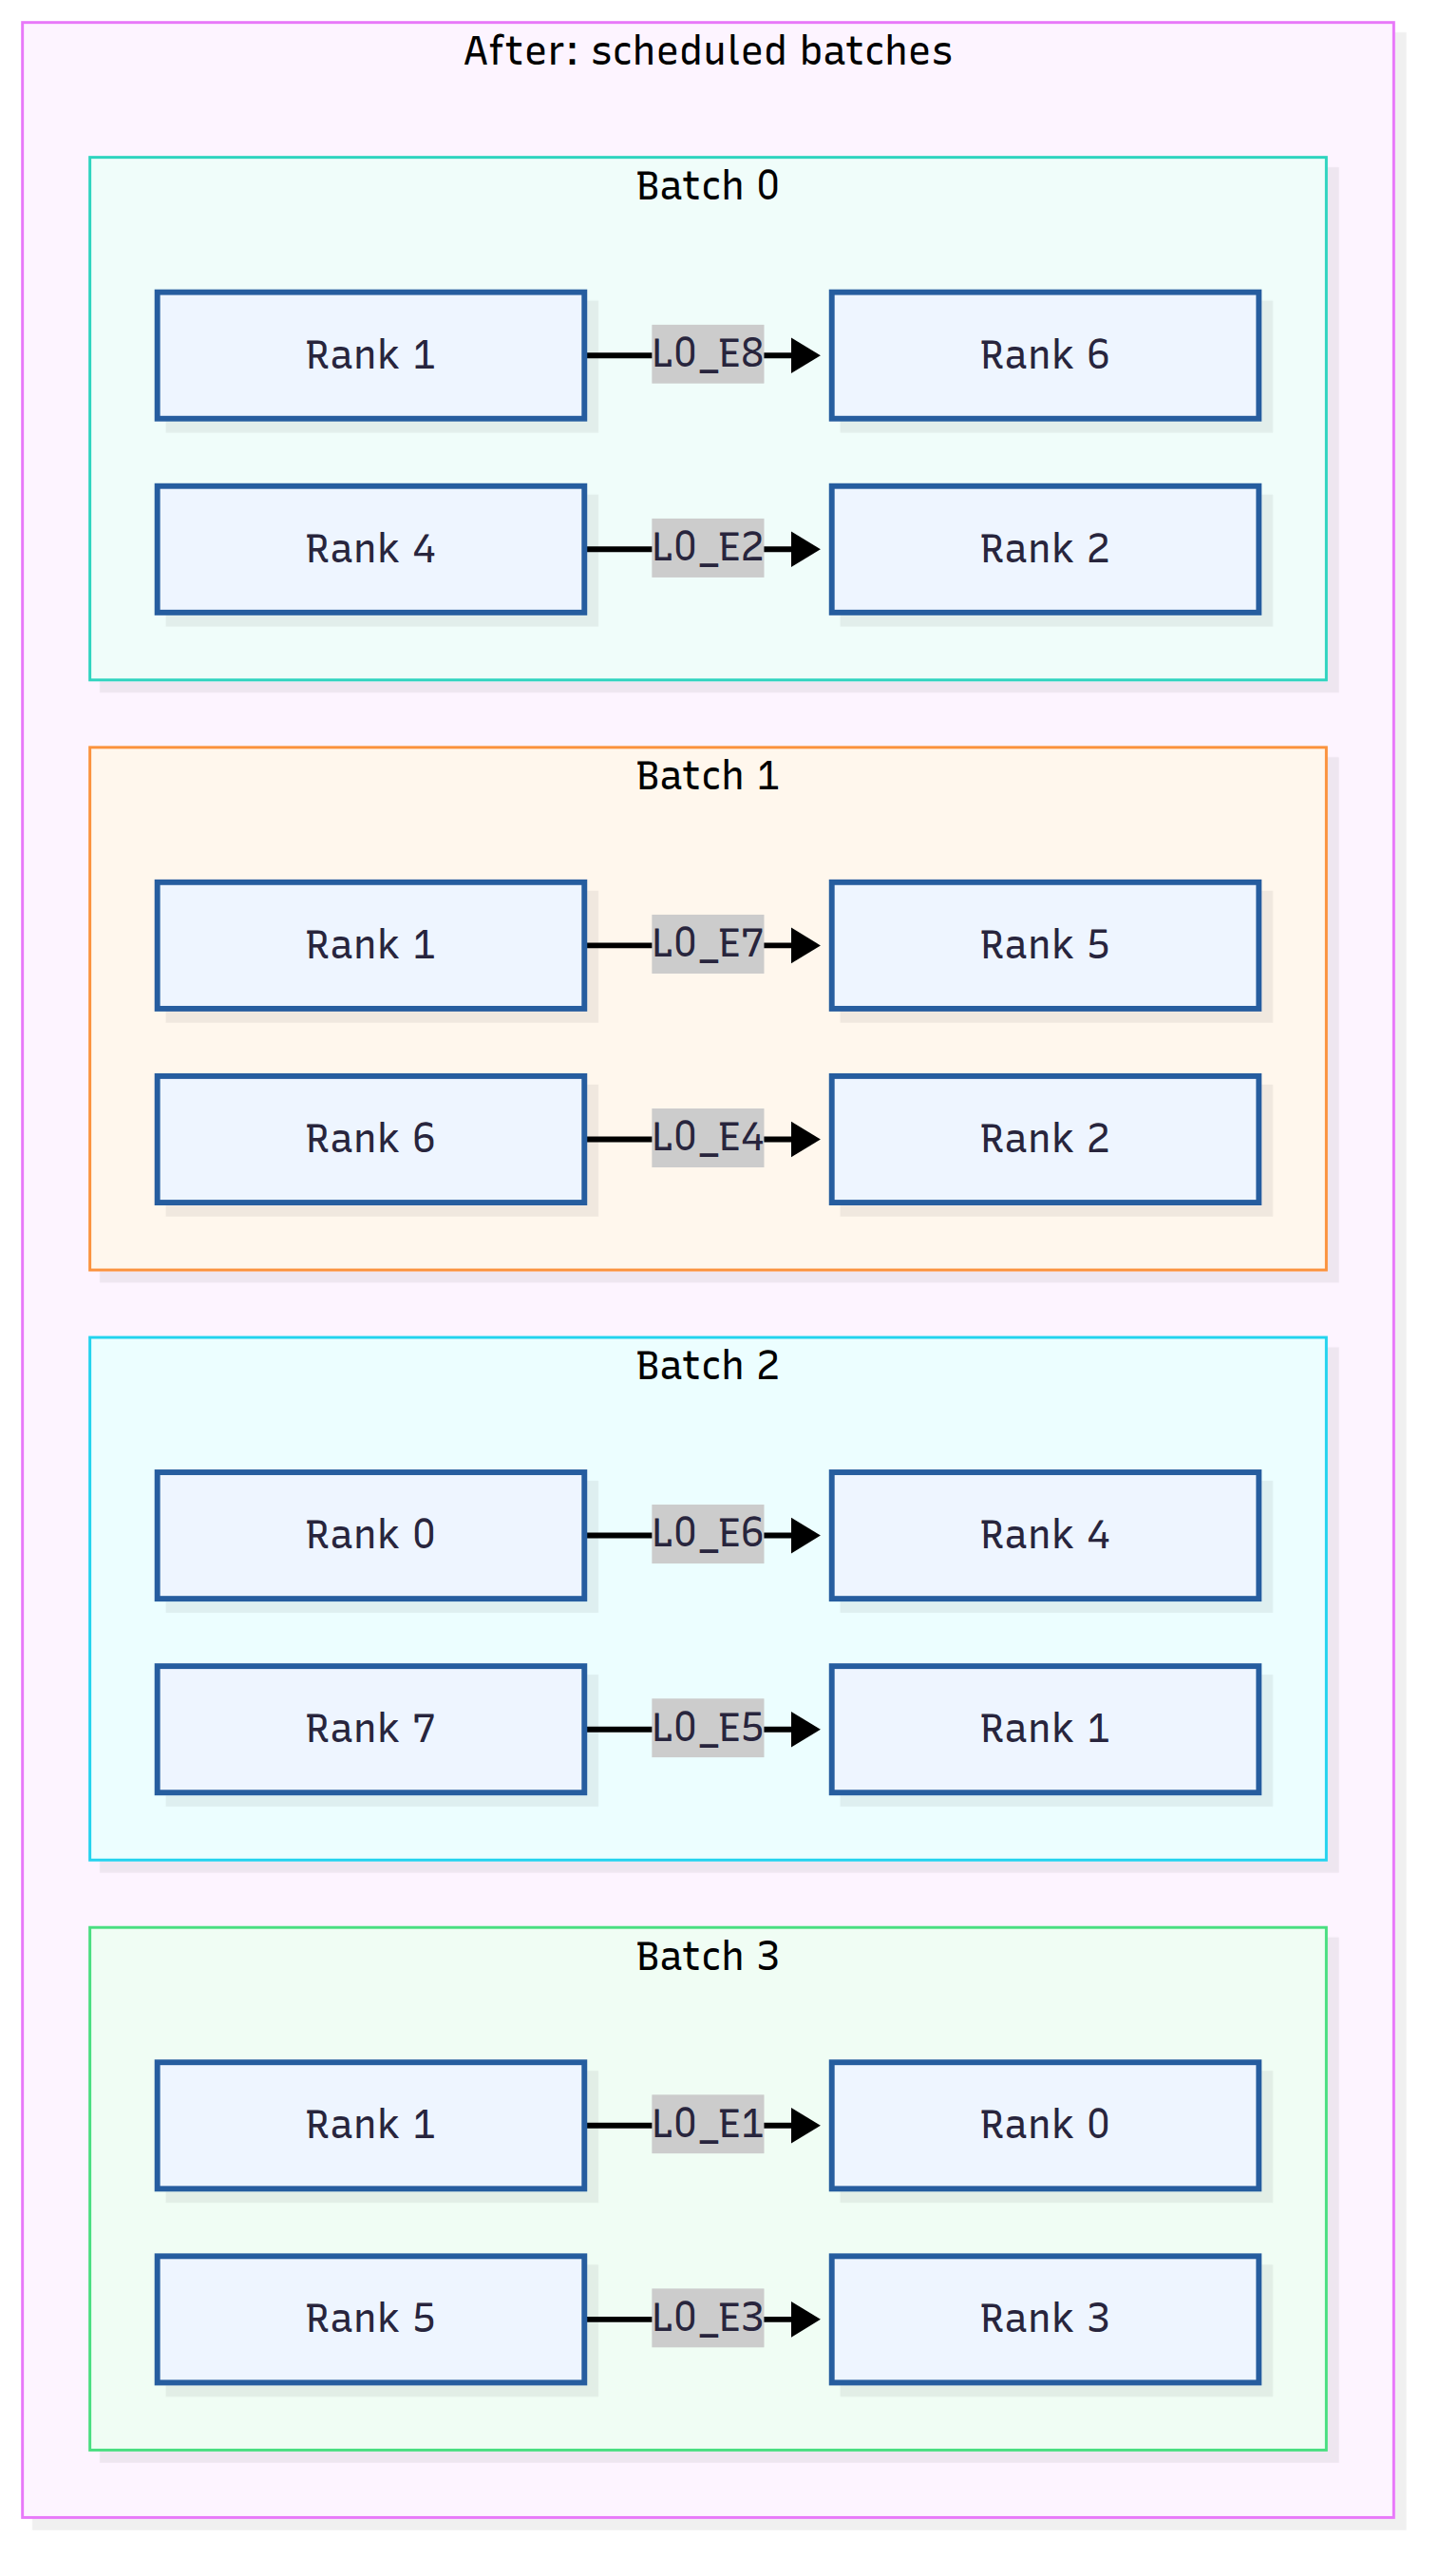
\includegraphics[width=\linewidth]{example_hotspot_after.png}
    \caption{ILP schedule split into batches.}
  \end{subfigure}
  \caption{Illustrative hotspot topology and migration schedules before and
  after contention-aware batching. The unbatched diagram remains a directed
  rank graph; only its layout is vertical.}
  \label{fig:ilp-before-after}
\end{figure}

\begin{table}[t]
  \centering
  \caption{Result of the illustrative ILP instance. Values are normalized.}
  \label{tab:ilp-result}
  \begin{tabular}{lrr}
    \toprule
    Metric & Unbatched & Constrained ILP optimum \\
    \midrule
    Modeled inference time & 4.75 & 2.25 \\
    Estimated migration time & 1.55 & 2.20 \\
    Peak link utilization & 1.50 & 0.50 \\
    Number of batches & 1 & 4 \\
    \bottomrule
  \end{tabular}
\end{table}

As shown in \cref{tab:ilp-result}, the constrained optimum reduces peak link utilization
by a factor of three and modeled inference time by more than half, but increases
estimated migration time and uses four batches. This result supplied the design
insight for the online scheduler: preserve parallelism between independent rank
pairs while explicitly limiting each rank's fan-in and fan-out within a batch.

\subsection{Why the ILP is not used online}

The optimizer is intentionally separated from the serving path. It is not an
``optimal implementation'' of EPLB: it is an exact offline reference for one
restricted mathematical formulation. First, an
online solver would add SciPy/HiGHS dependencies and variable solve latency to
a periodic control operation. Second, the latency model in
\cref{eq:slowdown} is an abstraction. Real interference depends on transport
protocols, queueing, CPU progress, message sizes, and simultaneous inference
collectives. An exact optimum of an approximate model is not necessarily a
better production choice than a conservative rule.

Third, all ranks already possess the placement maps needed to construct the
same deterministic schedule. A lightweight local algorithm avoids a new
coordination service. The ILP remains valuable for explaining the objective,
checking small instances, and motivating the endpoint constraint. The next
chapter derives the deployed algorithm from that constraint.


\chapter{Design and Implementation}
\label{ch:design}

\subsection{Design requirements}

The production design follows six requirements derived from the vLLM runtime.

\begin{enumerate}
  \item \textbf{Semantic preservation.} The same new placement must be reached
  as in the unbatched path. Scheduling may change transfer order, but not the
  selected logical experts, destination slots, or replica assignment.

  \item \textbf{No endpoint contention inside a batch.} Each rank participates
  in at most one coalesced directed flow, whether as sender or receiver.
  Independent rank pairs should remain concurrent.

  \item \textbf{Determinism.} Every rank builds the same batch structure from
  replicated placement arrays without exchanging a separate schedule.

  \item \textbf{Low control-plane cost.} The algorithm runs repeatedly during
  serving. It must avoid an optimizer and minimize Python object construction
  and repeated function-entry overhead.

  \item \textbf{Communicator compatibility.} Batch boundaries must be visible
  to the communication backend, and NIXL's transfer context lifecycle must be
  respected.

  \item \textbf{Safe rollout.} The new behavior is disabled by default and is
  reachable only in asynchronous EPLB. Existing synchronous users retain the
  established migration path.
\end{enumerate}

\subsection{From placements to remote flows}

For each rank, the scheduler converts its old and new local slot arrays into
sets of logical expert identifiers. The difference
$H^{\mathrm{new}}_r\setminus H^{\mathrm{old}}_r$ identifies experts that rank
$r$ must receive remotely. An expert already present locally does not generate
a remote instruction even when its physical row changes.

The algorithm then indexes old source ranks only for expert identifiers that
are needed somewhere. This filtering avoids building a global inverse index
for experts irrelevant to the current migration. If several source replicas
exist, the ordered destinations are divided evenly among them using quotient
and remainder assignment. This reproduces the legacy source-balancing logic.

Finally, expert identifiers are grouped in a dictionary keyed by
$(s,d)$. One \code{MigrationFlow} contains the source rank, destination rank,
and immutable tuple of experts for that ordered pair. Direction is retained for
send/receive execution, although the contention test treats both endpoints
symmetrically.

\subsection{Greedy rank-disjoint grouping}

The communication graph has rank vertices and one coalesced edge for each
directed pair. A batch is a matching. The scheduler processes flows in
deterministic insertion order and places each in the first existing batch whose
endpoint set is disjoint. If no batch is compatible, it creates a new one.

Instead of maintaining a Python set for every batch, the implementation uses an
integer bit mask. For a flow $(s,d)$,

\begin{equation}
  m_{s,d}=(1\ll s)\;\lor\;(1\ll d).
\end{equation}

If $u_b$ is the mask of ranks already used in batch $b$, the flow fits exactly
when $m_{s,d}\land u_b=0$. On insertion, $u_b$ becomes
$u_b\lor m_{s,d}$. This is constant-time endpoint testing for practical EP
group sizes.

\begin{algorithm}[t]
  \caption{Deterministic first-fit migration batching}
  \label{alg:greedy}
\begin{lstlisting}[style=code,mathescape=true]
Input: coalesced flows P in deterministic order
batches = []; used = []
for flow p = (src, dst, expert_ids) in P:
    mask = (1 << src) | (1 << dst)
    for batch_index in range(len(batches)):
        if mask & used[batch_index] == 0:
            batches[batch_index].append(p)
            used[batch_index] |= mask
            break
    else:
        batches.append([p])
        used.append(mask)
return batches
\end{lstlisting}
\end{algorithm}

The greedy algorithm does not promise the minimum number of colors for every
graph. That is acceptable because batch count is secondary to a simple and
conservative concurrency cap. On four ranks, a batch contains at most two
independent directed flows. The rank-disjoint rule intentionally leaves
headroom rather than trying to saturate the NIC with migrations. Reciprocal
flows such as $r_0\rightarrow r_1$ and $r_1\rightarrow r_0$ are distinct
directed flows and therefore occupy separate batches, even though they involve
the same rank pair.

\subsection{Correctness invariants}

The scheduler and execution path maintain three key invariants.

\paragraph{Completeness.}
Each remote gain appears in exactly one coalesced pair and each pair is inserted
in exactly one batch. Hence every derived migration is scheduled once.

\paragraph{Conflict freedom.}
Suppose two flows in the same batch share rank $r$. Both masks contain bit $r$.
When the second flow is considered, its mask intersects the batch mask, so the
algorithm rejects that batch. This contradicts co-residence; therefore flows in
a batch have disjoint endpoints.

\paragraph{Local-copy preservation.}
Experts already available on a destination rank are excluded before remote
flow construction. The existing local copy and receive-primary metadata still
control physical-row updates. Batching modifies only the remote communication
phase.

Unit tests cover deterministic grouping, rank-pair coalescing, random
instruction completeness, exclusion of local copies, replica balancing,
multi-layer equivalence, and execution with a mock communicator. The upstream
change added the test file to vLLM's expert-parallel CI area.

\subsection{Complexity}

Let $S$ be the number of physical slots across all ranks in one layer, $M$ the
number of remote expert migrations, $F$ the number of distinct directed rank
pairs after coalescing, and $K$ the number of produced batches. Placement
scanning is $O(S)$. Building and grouping the migrations is $O(M)$ expected
time with hash tables. First-fit placement is $O(FK)$ in the worst case and
$O(F)$ storage, in addition to the placement indices.

For a fixed small number of ranks, $K$ is bounded and the practical cost is
close to linear in placement size plus migration count. More importantly, the
implementation invokes the outer scheduler once for all layers in a rebalance
cycle. If the model contains $L$ MoE layers, it still constructs $L$
independent schedules, but avoids $L$ separate profiled entry points and
repeated surrounding Python setup.

\subsection{Cycle-wide precomputation, layer-wise transfer}

An earlier design called the scheduler immediately before each layer transfer.
The final design receives two-dimensional old and new placement arrays and
computes a list of schedules---one per layer---inside one cycle-wide call. This
does \emph{not} combine expert payloads from different layers. The asynchronous
worker later iterates over layers and passes only the corresponding schedule to
the transfer function.

The distinction is important. Weight transfers and mapping activation preserve
the existing layer lifecycle, limiting memory and synchronization changes.
Only CPU schedule construction is aggregated. Qwen3-30B-A3B has 48 layers, so
one profiling range represents schedule construction for all 48 layers. The
worker waits for the new placement maps before this step; adding a few
milliseconds of CPU work once per rebalance cycle is negligible relative to
the measured cycle interval, but this claim is verified rather than assumed in
\cref{sec:profile-results}.

\subsection{Batched execution}

For a layer, the executor first creates maps from logical expert identifier to
the old and new local physical row. It then processes the ordered list of
batches. For every batch it:

\begin{enumerate}
  \item restores the communicator's transfer context for the current old
  placement and layer;
  \item posts sends for flows whose source is the local EP rank;
  \item posts receives into expert buffers for flows whose destination is the
  local EP rank; and
  \item calls \code{communicator.execute()} to preserve the batch boundary.
\end{enumerate}

For NIXL, restoring context per batch is required because execution drains the
queued operations and clears the transfer context. Calling \code{execute()}
once after all batches would submit the operations together, erasing the very
boundaries that enforce rank-disjoint concurrency. Conversely, an uninvolved
rank can have no send or receive in a given batch; the backend and existing
layer coordination govern progress.

\subsection{Configuration and failure containment}

The change adds \code{enable\_migration\_batching} to \code{EPLBConfig}, with
default \code{false}. The effective property is

\begin{equation}
  \texttt{migration\_batching\_enabled}
  =\texttt{use\_async}\land\texttt{enable\_migration\_batching}.
\end{equation}

Thus, setting the new flag cannot alter synchronous EPLB. This is a deliberate
engineering boundary. In synchronous mode, serving is stopped and serial
batches can only delay its resumption. In asynchronous mode, the operator can
enable batching when network interference is a concern. Keeping the feature
opt-in also acknowledges that the current evidence comes from one cluster and
that the optimal concurrency limit may vary with topology.

When disabled, the original path constructs local metadata, posts all remote
sends and receives, and invokes the communicator once. The feature does not
change model routing, balancing policy, or numerical output. This small impact
surface was important for upstream review and made rollback a configuration
change rather than a code revert.

\subsection{Upstream integration}

The final patch added a scheduler module, unit tests, one configuration field,
async-worker wiring, and a batched branch in the migration executor. It did not
ship the offline ILP, datasets, experimental scripts, or thesis artifacts as
runtime dependencies. The contribution was merged into vLLM on 3 October 2026
as pull request \prnumber\ \cite{vllmpr52641}. The separation between research
artifacts and production files keeps the upstream change reviewable and avoids
coupling online serving to the experimental environment.


\chapter{Experimental Methodology}
\label{ch:methodology}

\subsection{Evaluation goals}

The experiments answer three operational questions:

\begin{enumerate}
  \item Does enabling migration batching improve user-visible serving metrics
  under asynchronous EPLB?
  \item Does it reduce high-percentile network traffic, the mechanism the
  scheduler is designed to affect?
  \item Is the CPU scheduling overhead small relative to the observed E2E time
  saved?
\end{enumerate}

These questions lead to three directional expectations rather than formal
statistical hypotheses. First, batching should lower the high tail of observed
NIC traffic because fewer migration flows contend at one rank. Second, if that
reduction protects foreground communication, output throughput should increase
and TTFT, TPOT, and E2E latency should decrease. Third, cycle-wide schedule
construction should consume only a small fraction of the serving time saved.
The single A/B pair can check whether the observations have these directions,
but it cannot establish significance or estimate run-to-run variance.

Two separate runs are used for two separate purposes. A clean A/B serving run
compares batching off and on without profiler instrumentation. A profiling run
repeats the batching-on condition with NVTX-only Nsight Systems capture. This
separation prevents profiler overhead from contaminating the reported serving
comparison.

\subsection{Hardware and software environment}

\begin{table}[t]
  \centering
  \caption{Experimental environment.}
  \label{tab:environment}
  \begin{tabularx}{\textwidth}{lX}
    \toprule
    Component & Configuration \\
    \midrule
    Nodes & Four Ubuntu 22.04.5 servers \\
    Accelerators & One NVIDIA Quadro RTX 6000, \SI{24}{GB}, per node \\
    Network & \SI{10}{Gb/s} Ethernet, interface \code{eno2}, no RDMA \\
    Model & Qwen/Qwen3-30B-A3B-Instruct-2507, FP16 \\
    Parallelism & Tensor parallel size 4; expert parallel enabled \\
    Runtime & Experimental vLLM build; Ray 2.56.1 \\
    Migration backend & NIXL 1.3.2 over UCX/TCP \\
    Execution & Eager mode; prefix caching enabled \\
    Profiling & NVIDIA Nsight Systems 2024.5.1, NVTX-only \\
    \bottomrule
  \end{tabularx}
\end{table}

The four GPU processes serve as both TP and EP ranks. One GPU per host makes
each inter-rank expert transfer an inter-node transfer, avoiding ambiguity
between local NVLink/PCIe movement and Ethernet traffic. The hardware is not a
modern production cluster; its relatively constrained network is useful for
observing contention but limits external validity.

NCCL and Gloo are bound to \code{eno2}, InfiniBand is disabled, and UCX is
also bound to the same device. NIXL is selected explicitly rather than relying
on automatic backend selection. Both A/B conditions use the same software
revision and network configuration.

\subsection{Model and EPLB configuration}

The evaluated model contains 48 layers and 128 experts, selecting eight experts
per token \cite{qwen3modelcard}. Server maximum sequence length is 4096 and GPU
memory utilization is set to 0.9. EPLB uses the configuration in
\cref{tab:eplb-config}.

\begin{table}[t]
  \centering
  \caption{EPLB parameters common to the A/B experiment.}
  \label{tab:eplb-config}
  \begin{tabular}{lr}
    \toprule
    Parameter & Value \\
    \midrule
    \code{window\_size} & 50 \\
    \code{step\_interval} & 50 \\
    \code{num\_redundant\_experts} & 32 \\
    \code{log\_balancedness} & false \\
    \code{use\_async} & true \\
    \code{communicator} & \code{nixl} \\
    \code{enable\_migration\_batching} & false / true \\
    \bottomrule
  \end{tabular}
\end{table}

The short observation and step intervals deliberately cause recurring
rebalances during the finite benchmark. This is a stress-oriented configuration
for studying the migration path rather than a recommended production default.
The 32 redundant experts create physical flexibility for EPLB to react to
recent routing demand.

\subsection{Workload}

Each condition starts a fresh server and executes an eight-request warm-up.
The measured workload uses \code{vllm bench serve} with 500 successful requests
and maximum concurrency 32. Every request has a 300-token random prefix, 200
additional input tokens, and 300 requested output tokens. The random seed is
zero, temperature is zero, and end-of-sequence tokens are ignored so all
requests produce the configured output length. Prefix caching remains enabled,
matching the intended online configuration rather than disabling cache to
manufacture compute load.

The request set is synthetic. It controls sequence lengths and makes the A/B
conditions comparable, but random tokens are not representative of semantic
production traffic. The experiment studies system interference under frequent
migration, not application-level output quality. Because placement batching
does not modify model computation or routing decisions, no accuracy evaluation
is required for the feature itself.

\subsection{A/B procedure and controls}

The independent variable is
\code{enable\_migration\_batching}. All other documented parameters are held
constant. The off case ran first and the on case second, each with a fresh
server. Both completed 500 of 500 requests with zero failures. The benchmark
client records aggregate duration and request-level latency distributions.

The experiment is a single repetition. It therefore cannot quantify run-to-run
variance, confidence intervals, or statistical significance. Percent changes
are descriptive comparisons of these archived runs. A stronger study would
randomize condition order and repeat each condition enough times to estimate
variance. This limitation is stated explicitly rather than obscured by the
large number of requests, because requests within one long run are not
independent replications of server startup and cluster state.

\subsection{Serving metrics}

For a metric where larger is better, such as throughput, improvement is

\begin{equation}
  I_{\uparrow}=\frac{V_{\mathrm{on}}-V_{\mathrm{off}}}
  {V_{\mathrm{off}}}\times100\%.
\end{equation}

For a latency metric where smaller is better,

\begin{equation}
  I_{\downarrow}=\frac{V_{\mathrm{off}}-V_{\mathrm{on}}}
  {V_{\mathrm{off}}}\times100\%.
\end{equation}

The thesis reports output tokens per second and P50/P99 TTFT, TPOT, and E2E
latency. Request throughput is retained in the raw JSON and the supplementary
table. Because all 500 requests produce exactly 300 output tokens, request and
output throughput necessarily have the same relative change; the main text
uses output throughput to avoid presenting this one result twice. P99 values
are computed by the benchmark client from the 500 request samples.

\subsection{NIC measurement}

NIC traffic is not produced by \code{vllm bench serve}. A separate sampler on
the head node reads the cumulative receive and transmit byte counters under
\path{/sys/class/net/eno2/statistics/} once per second. For adjacent samples at
times $t_{i-1}$ and $t_i$, aggregate traffic is

\begin{equation}
  B_i=\frac{(RX_i-RX_{i-1})+(TX_i-TX_{i-1})}
  {t_i-t_{i-1}}.
\end{equation}

Values are converted to MB/s and the P99 is computed over the formal benchmark
window. Summing RX and TX describes total head-node interface pressure; it is
not physical link utilization and it cannot attribute bytes to EPLB versus
inference. The A/B comparison and time-series shape provide supporting evidence,
not packet-level causal attribution.

\subsection{Scheduler profiling}

The profiling run uses the same model, EPLB settings, workload lengths,
concurrency, and 500 prompts as the batching-on E2E condition. The only change
is that Ray processes are launched in NVTX-only Nsight Systems sessions with
CPU sampling and context-switch tracing disabled. NVTX ranges are designed to
mark application phases with low capture volume \cite{nsightguide}.

The range \code{eplb: schedule migration batches} encloses the call that builds
schedules for all 48 layers. Each rank writes its own \code{rank*.nsys-rep}.
Explicit formal-start and formal-end timestamps exclude model loading and
warm-up. The reports were analyzed with Nsight Systems 2024.5.1. For each rank,
the number of calls, P50 and P99 elapsed duration per call, and cumulative
duration are extracted.

The explicit CUDA NVTX range was temporary measurement instrumentation added
only to make the asynchronous EPLB worker visible to Nsight Systems. It was
used in the profiling run, was absent from the clean E2E A/B run, and was not
included in the final production patch. The scheduler call and placement
inputs were otherwise unchanged.

Ranks construct their identical schedules concurrently on different host
CPUs. Their costs must therefore not be summed to estimate critical-path
overhead. A conservative comparison uses the largest cumulative rank cost,
$C_{\max}$, and clean A/B time saved,

\begin{equation}
  S=T_{\mathrm{off}}-T_{\mathrm{on}}.
\end{equation}

The cost-to-saved ratio is

\begin{equation}
  R=\frac{C_{\max}/1000}{S}\times100\%.
  \label{eq:cost-ratio}
\end{equation}

This ratio does not claim that all scheduling time lies on the serving critical
path. It intentionally compares a directly measured conservative CPU elapsed
cost with the directly measured wall-clock difference.

\subsection{Data provenance and reproducibility}

The authoritative E2E source directory is
\path{results/serving_nixl_20260911_async_random500}. It contains the
unmodified off/on \code{bench.json}, server and client logs, EPLB
configuration, one-second \code{nic.tsv}, warm-up output, plotting source, and
summary CSV files. The authoritative profiling directory is the same name with
suffix \code{\_profile}; it contains four Nsight reports, formal-window
timestamps, benchmark output, exact commands, and \code{profile\_summary.csv}.

Older directories represent intermediate designs or exploratory workloads and
are excluded from all final tables. Reproduction commands are transcribed in
\cref{app:commands}. This explicit provenance prevents accidental selection of
a favorable intermediate run.


\chapter{Results and Discussion}
\label{ch:results}

\section{End-to-end serving results}

\Cref{tab:e2e-results} reports the clean A/B measurement. Both conditions
completed all 500 requests. Enabling batching shortened total benchmark
duration from \SI{4756.098}{s} to \SI{4650.166}{s}, a difference of
\SI{105.932}{s}. Output throughput increased from 31.54 to 32.26 tokens/s, or
2.28\%.

\begin{table}[p]
  \centering
  \caption{End-to-end serving results. Lower is better for all latency
  columns; higher is better for throughput. Each condition is one run.}
  \label{tab:e2e-results}
  \resizebox{\textwidth}{!}{%
  \begin{tabular}{lrrrrrrr}
    \toprule
    Batching & Duration (s) & Output tok/s &
    TTFT P50 & TTFT P99 & TPOT P50 & TPOT P99 & E2E P50 / P99 \\
    \midrule
    Off & 4756.10 & 31.54 & 49180.71 & 75740.25 & 828.53 & 1007.82 & 303462.69 / 322184.88 \\
    On  & 4650.17 & 32.26 & 48599.04 & 74756.17 & 812.44 & 999.01 & 293821.76 / 317351.61 \\
    \bottomrule
  \end{tabular}}
  \vspace{1mm}

  \footnotesize Latency values are milliseconds.
\end{table}

All six reported latency percentiles moved in the favorable direction.
Median/P99 TTFT decreased by 1.18\%/1.30\%; median/P99 TPOT decreased by
1.94\%/0.87\%; and median/P99 E2E latency decreased by 3.18\%/1.50\%.
The larger improvement in median E2E than in an individual TTFT or TPOT
percentile should not be interpreted as an algebraic sum of percentile changes:
each percentile may correspond to a different request, and E2E accumulates
many decode intervals.

\begin{figure}[t]
  \centering
  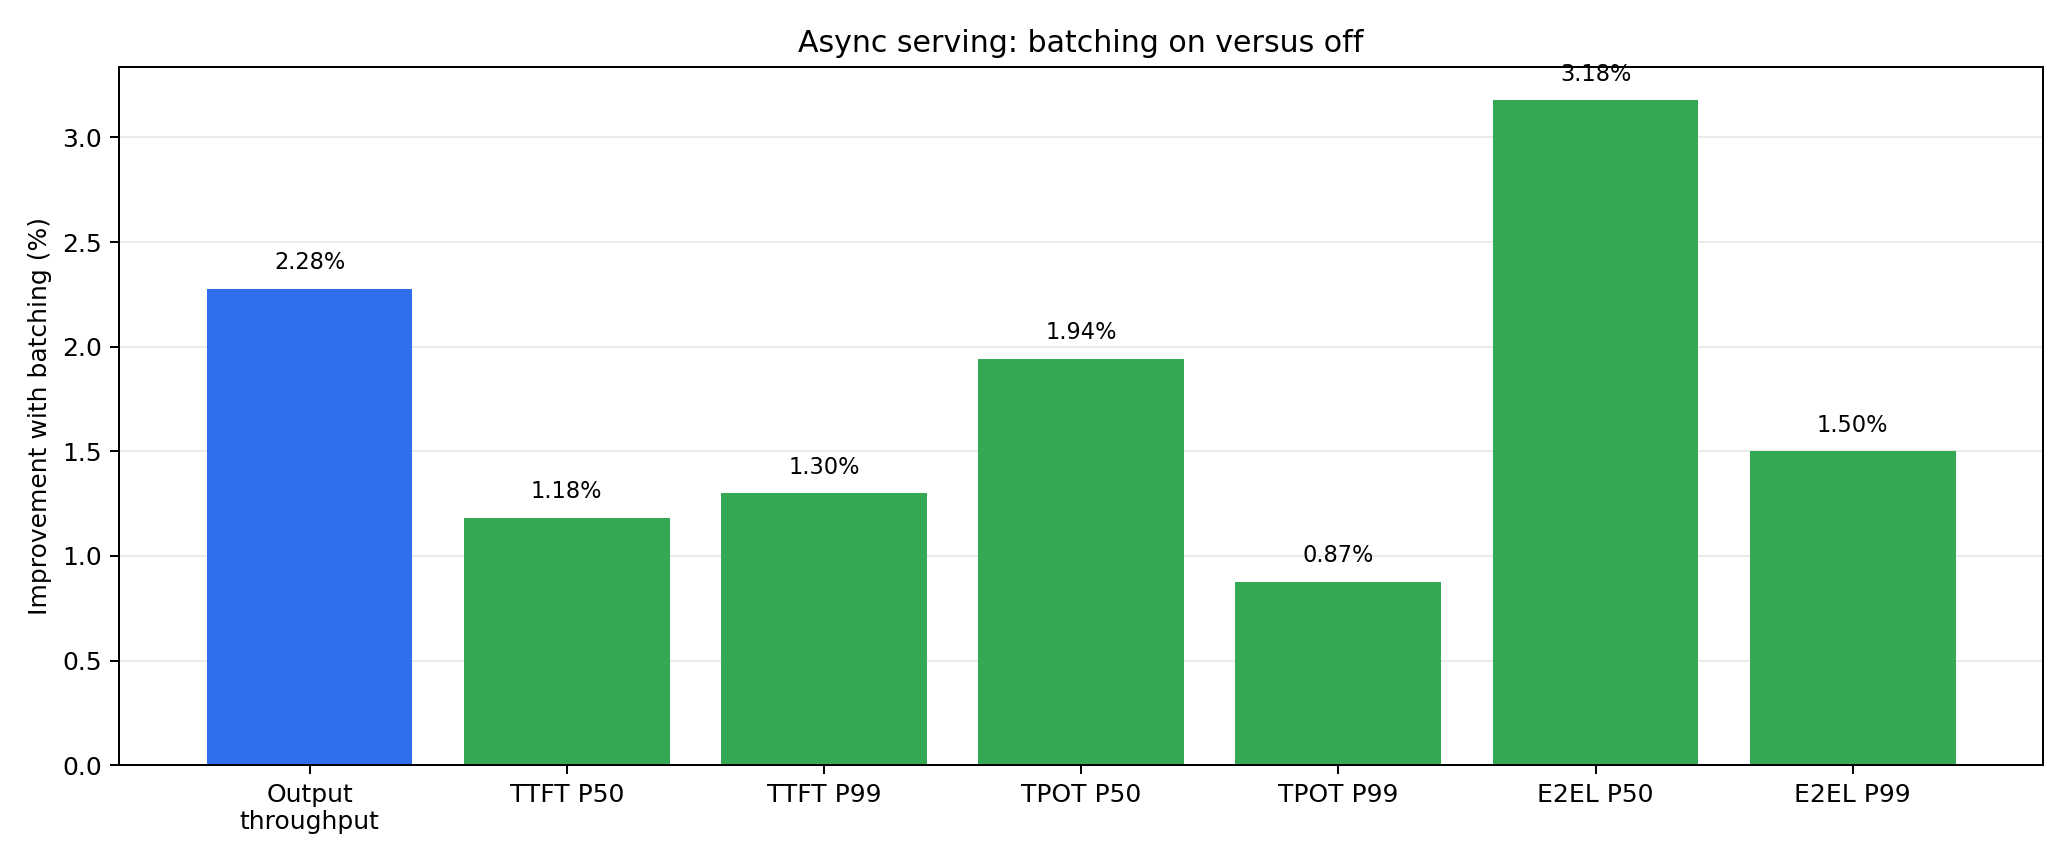
\includegraphics[width=0.92\textwidth]{e2e_improvement.png}
  \caption{Relative improvement with batching enabled in the clean A/B run.
  Positive values indicate higher throughput or lower latency.}
  \label{fig:e2e-improvement}
\end{figure}

The direction is consistent with the hypothesis that migration bursts interfere
with inference. TTFT improves despite batching being a background migration
optimization because the benchmark mixes prefill and decode across concurrent
requests. TPOT improves because decode continues throughout asynchronous
migration. The result does not isolate which inference communication operation
benefited; it measures the user-visible aggregate effect.

\section{Network traffic}

The head-node P99 of aggregate RX+TX traffic decreased from 599.81 MB/s to
538.40 MB/s, a reduction of 10.24\%. This is the largest relative change among
the reported measurements and directly concerns the mechanism targeted by the
scheduler: smoothing extreme network demand rather than reducing total expert
bytes.

\begin{figure}[p]
  \centering
  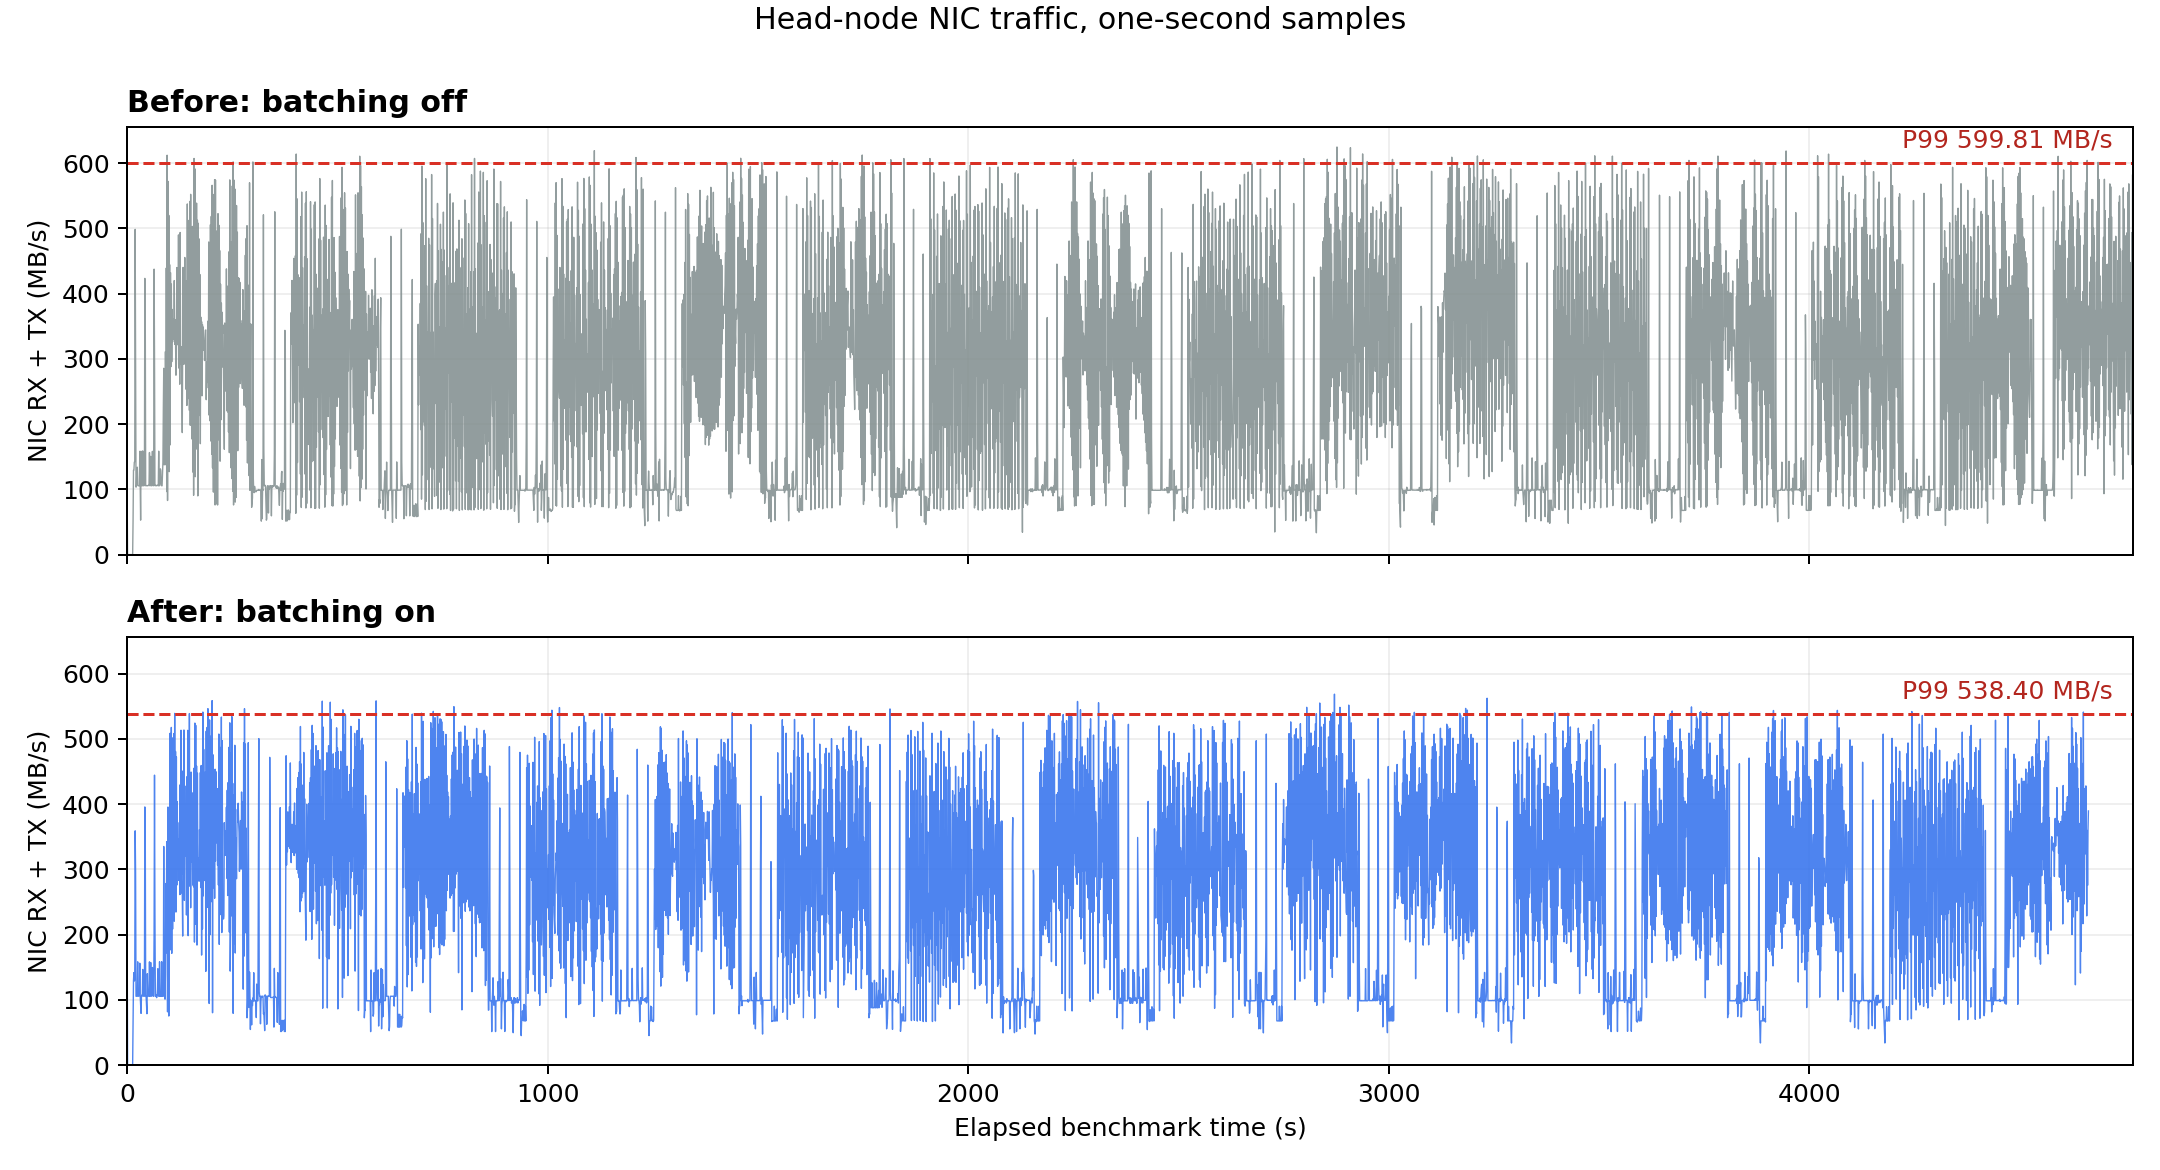
\includegraphics[width=\textwidth]{nic_timeseries.png}
  \caption{Head-node aggregate NIC traffic sampled once per second during the
  two independent runs. Batching reduces the high tail of observed traffic.}
  \label{fig:nic-series}
\end{figure}

\Cref{fig:nic-series} shows that traffic is bursty in both configurations.
This is expected: inference itself communicates and EPLB continues to migrate
whole expert tensors. The scheduler does not impose a byte-rate limiter. It
limits per-rank flow concurrency, spreading conflicting migration flows across rounds.
The lower P99 supports the contention explanation, but the two time series are
not temporally aligned executions of identical low-level events. They are
separate A/B runs with the same client workload.

The measurement also has a scope limitation. Only the head node was sampled,
so the result does not prove that every worker's P99 decreased. Because the
scheduler enforces the same rank-degree constraint globally, lower bursts are
plausible on other ranks, but per-node counters are necessary to verify that
claim.

\section{Scheduler profiling}
\label{sec:profile-results}

All four ranks recorded 34 calls to the cycle-wide scheduling range during the
formal profiling window. Since one call prepares all 48 layer schedules, the
trace represents 34 rebalance-cycle scheduling events per rank, not
$34\times48$ independent top-level calls.

\begin{table}[t]
  \centering
  \caption{NVTX elapsed time for cycle-wide scheduler calls.}
  \label{tab:profile}
  \begin{tabular}{rrrrr}
    \toprule
    Rank & Calls & P50/call (ms) & P99/call (ms) & Cumulative (ms) \\
    \midrule
    0 & 34 & 7.819 & 17.536 & 302.081 \\
    1 & 34 & 7.090 & 12.357 & 253.152 \\
    2 & 34 & 7.035 & 16.104 & 255.239 \\
    3 & 34 & 7.005 & 8.103  & 241.190 \\
    \bottomrule
  \end{tabular}
\end{table}

Median elapsed time is between 7.01 and 7.82 ms per rank per rebalance cycle.
Dividing by 48 gives roughly 0.146--0.163 ms per layer as an intuition, but the
implementation and profiler measure one aggregated call, so this quotient is
not presented as an independently observed per-layer latency. P99 variability
is larger, consistent with host scheduling and interference in the background
thread.

Rank 0 has the largest cumulative cost, \SI{302.081}{ms}. Ranks execute on
separate hosts and schedule concurrently, so adding the four cumulative values
would overstate wall-clock overhead. Applying \cref{eq:cost-ratio} to the clean
A/B saving gives

\begin{equation}
  R=\frac{0.302081}{4756.098161-4650.165779}\times100\%
   =0.285\%.
\end{equation}

\begin{figure}[t]
  \centering
  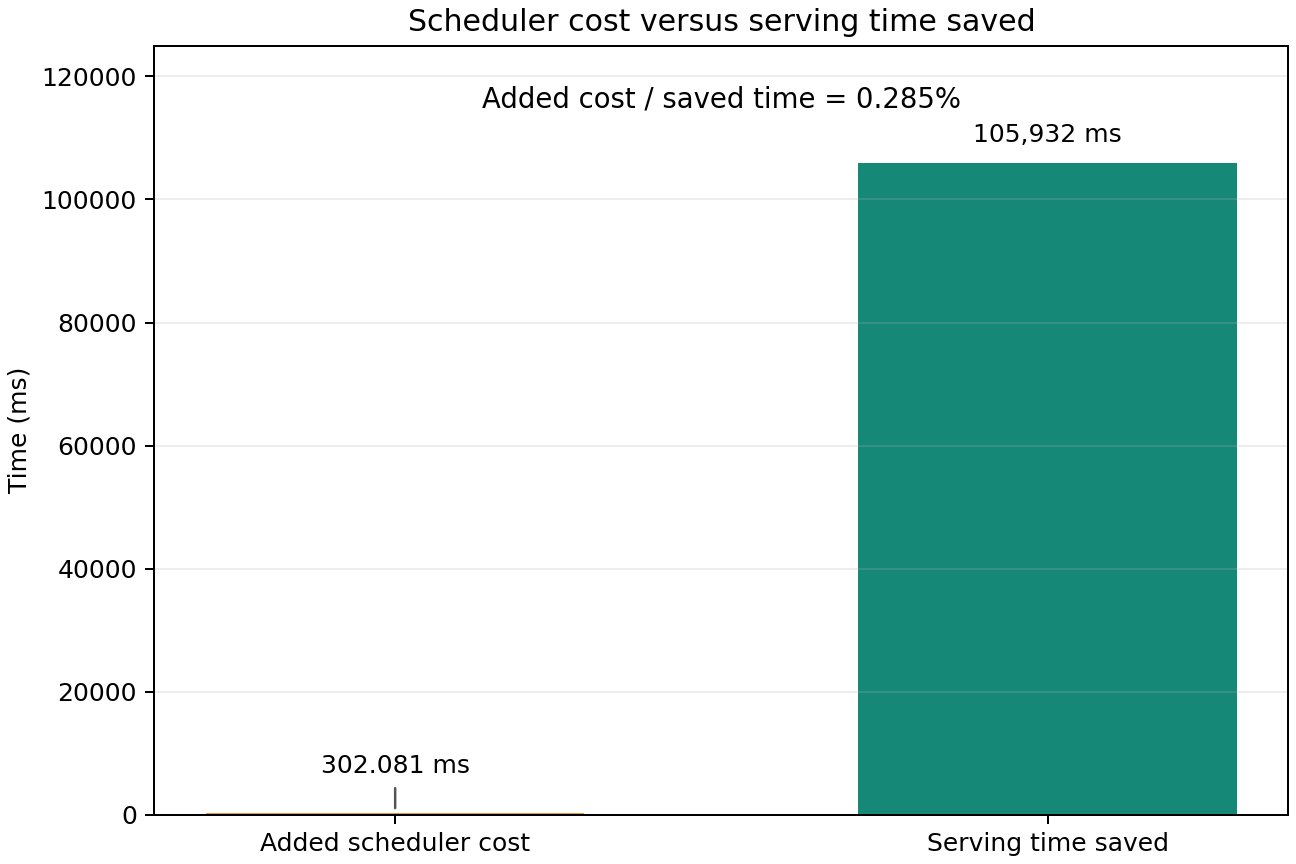
\includegraphics[width=0.82\textwidth]{scheduler_cost_vs_saved.png}
  \caption{Largest measured cumulative scheduler time versus serving time
  saved. The linear axis intentionally preserves the scale difference.}
  \label{fig:cost-saved}
\end{figure}

This comparison shows that the measured scheduler cost is small relative to
the observed completion-time difference. It is not a causal decomposition of
the saving: the profiler run is separate, and the 105.932 s difference includes
all downstream effects. It nevertheless answers the maintainer-facing systems
question of whether the additional Python scheduling work is of the same order
as the apparent benefit. It is not.

\section{Answering the research questions}

\paragraph{RQ1: representation.}
The directed migration-flow graph captures endpoint contention cleanly, while
the topology-aware ILP adds routed-link capacity for offline reasoning. The ILP
example confirms that minimizing foreground contention can intentionally
increase migration completion time.

\paragraph{RQ2: online scheduling.}
Coalescing by directed rank pair followed by first-fit edge coloring provides a
deterministic and dependency-free rule. The bit-mask representation makes the
central constraint explicit and inexpensive. It is not guaranteed to minimize
batch count, but exact color optimality is not required for safe throttling.

\paragraph{RQ3: semantic integration.}
Tests show completeness, conflict freedom, local-copy exclusion, replica
balancing, deterministic output, and correct mock-communicator execution. The
implementation restores NIXL context and executes each batch separately,
precomputes all layer schedules once per cycle, and leaves synchronous and
disabled paths unchanged.

\paragraph{RQ4: serving impact.}
In the evaluated cluster, every reported throughput or latency metric improved,
and NIC P99 decreased by 10.24\%. Scheduler profiling found a conservative
cost-to-saved ratio of 0.285\%. These results are consistent with reduced
migration interference and justify the implementation for this environment.

\section{Discussion}

The results illustrate why migration duration alone is the wrong optimization
target for asynchronous EPLB. A scheduler can add communication rounds yet
improve total serving completion time, because the foreground model continues
to execute during those rounds. The relevant resource is not only bytes moved
but how aggressively those bytes are injected while latency-sensitive traffic
is active.

The rank-disjoint-flow constraint is deliberately conservative. On $n$ ranks,
at most $\lfloor n/2\rfloor$ independent directed flows appear in a batch. A
topology-aware scheduler might safely allow greater rank participation when
ranks are co-located, use separate NICs, or have available bandwidth. The
fixed rule trades peak migration speed for predictable behavior and
portability without topology discovery.

Cycle-wide precomputation addresses a different concern: CPU overhead. It does
not make network batches coarser and does not transfer 48 layers together. It
reduces top-level scheduling invocations while preserving layer-wise migration.
This separation between scheduling granularity and transfer granularity is a
key engineering result of the work.

\section{Threats to validity}

\subsection{Internal validity}

The off run preceded the on run, so temporal drift, thermal state, background
load, or network state may contribute to the difference. Fresh servers and an
identical warm-up reduce but do not eliminate these effects. Only one run per
condition was retained; repeated interleaved runs would provide stronger
evidence. The client uses the same seed, yet stochastic system scheduling means
request timing is not identical.

NIC counters include all interface traffic. They cannot distinguish NIXL
migration bytes from Ray control traffic, model communication, or unrelated
traffic. A packet or transport-level trace and counters on every node would
strengthen causal attribution. Still, the lower NIC P99 and favorable serving
metrics are mutually consistent.

\subsection{Construct validity}

The ILP slowdown equation is a deliberately linear surrogate. Queueing and
protocol effects are nonlinear, and flow weights count experts rather than
bytes or measured transfer time. The ILP result should therefore be read as a
design demonstration. The E2E benchmark, not the ILP objective value, is the
evidence for real serving behavior.

The random-token workload fixes lengths and activates frequent EPLB, but it is
not a production request distribution. Ignoring EOS makes output work
deterministic but removes natural variation. Prefix caching is enabled, which
improves realism relative to disabling it, although random prefixes offer
limited sharing.

\subsection{External validity}

The cluster has four older GPUs and \SI{10}{Gb/s} Ethernet without RDMA.
Production systems may use NVLink within nodes and 100--400 Gb/s RDMA between
nodes. Higher bandwidth can reduce contention, whereas larger models and more
ranks can increase the number and size of migrations. Results may therefore be
smaller or larger in another environment.

Only Qwen3-30B-A3B-Instruct-2507 and NIXL 1.3.2 were used in the final study.
The code supports the vLLM communicator abstraction, but backend-specific
progress and synchronization behavior can change batch overlap. Separate
evaluation is needed for Gloo and future NIXL versions.

\subsection{Conclusion validity}

The results are effect estimates from a single A/B pair, not confidence
intervals. The thesis consequently avoids terms such as ``statistically
significant'' and does not generalize the exact percentages. The strongest
supported conclusion is conditional: under this documented configuration,
batching coincided with lower NIC tail traffic and improvements in all reported
serving metrics at a small measured scheduling cost.


\chapter{Conclusions and Future Work}
\label{ch:conclusions}

This thesis investigated a narrow systems problem created by dynamic expert
placement: how to migrate expert weights without allowing background network
traffic to interfere unnecessarily with ongoing inference. The key conceptual
step was to distinguish migration completion time from foreground serving
quality. In synchronous EPLB, finishing the migration quickly is appropriate
because inference is paused. In asynchronous EPLB, inference and migration
share resources, so lower peak contention can be worth additional transfer
rounds.

An offline ILP formalized this trade-off using flow-to-batch assignments,
rank-degree constraints, routed link load, and a worst-case inference-time
surrogate. It computes a constrained optimum after imposing the same
rank-disjoint-flow policy as the deployed design; it does not establish that
this concurrency limit is universally optimal. In an illustrative hotspot, the
constrained schedule reduced normalized
peak utilization from 1.5 to 0.5 and modeled inference time from 4.75 to 2.25,
while increasing estimated migration time from 1.55 to 2.20. The purpose of the
model was explanatory: it established that the apparent contradiction between
``more batches'' and ``faster serving'' disappears when the objectives are
separated.

The deployed scheduler translates that insight into deterministic first-fit
edge coloring. Remote migrations are coalesced by ordered rank pair, and every
batch forms a matching in the rank communication graph. Independent pairs
retain concurrency, but no rank participates in multiple directed flows within
a batch.
All layer schedules are constructed in one cycle-wide CPU call, while expert
weights remain transferred and activated layer by layer. The implementation is
opt-in, async-only, and preserves the legacy path as a safe fallback.

On the evaluated four-node vLLM system, enabling batching improved output
throughput by 2.28\%, reduced TTFT P50/P99 by 1.18\%/1.30\%, reduced TPOT
P50/P99 by 1.94\%/0.87\%, and reduced E2E P50/P99 by 3.18\%/1.50\%. Head-node
NIC P99 fell by 10.24\%. Profiling measured 34 scheduling calls for all 48
layers per rank, with \SI{302.081}{ms} as the largest cumulative rank cost.
That cost was 0.285\% of the independently observed \SI{105.932}{s} serving-time
reduction. The code was merged upstream into vLLM in pull request \prnumber.

The work also has clear limitations. It reports a single A/B pair on one
cluster, uses a synthetic random workload, samples NIC traffic on only the head
node, and evaluates one migration backend. Accordingly, the result is an
engineering case study rather than a universal throughput claim.

Several extensions follow naturally:

\begin{itemize}
  \item repeat and randomize A/B runs on server-class GPUs and RDMA networks,
  reporting confidence intervals and per-node network counters;
  \item relax the one-flow-per-rank limit using observed foreground load or
  available bandwidth rather than fixing it statically;
  \item incorporate topology, heterogeneous expert sizes, and multiple NICs
  while retaining a deterministic fallback;
  \item evaluate synchronization semantics and benefit across every supported
  communicator backend;
  \item coordinate placement and migration scheduling so a placement policy can
  account for reconfiguration cost without coupling model routing to a complex
  online optimizer; and
  \item expose migration progress and interference metrics for automatic
  operator tuning.
\end{itemize}

The broader lesson is that online model reconfiguration should be evaluated as
part of serving, not as an isolated data-transfer benchmark. A migration that
finishes later can still be the better systems choice when it protects the
latency and throughput of user requests.


\addtocontents{toc}{\vspace{2em}}
\bibliography{Thesis_bibliography}

\cleardoublepage
\addtocontents{toc}{\vspace{2em}}
\appendix
\chapter{Reproduction Commands}
\label{app:commands}

This appendix records the essential final commands. The archived
\code{COMMANDS.md} files remain the authoritative machine-readable source.

\section{Environment and server}

\begin{lstlisting}[style=code,language=bash]
export NCCL_IB_DISABLE=1 NCCL_SOCKET_FAMILY=AF_INET
export NCCL_SOCKET_IFNAME=eno2 GLOO_SOCKET_IFNAME=eno2
export UCX_TLS=all UCX_NET_DEVICES=eno2
export UCX_RCACHE_MAX_UNRELEASED=1024
export VLLM_EPLB_LOG_MIGRATION_STATS=0

MODEL=Qwen/Qwen3-30B-A3B-Instruct-2507
USE_BATCHING=true  # repeat with false
EPLB_CONFIG="{\"window_size\":50,\"step_interval\":50,\
\"num_redundant_experts\":32,\"log_balancedness\":false,\
\"use_async\":true,\"communicator\":\"nixl\",\
\"enable_migration_batching\":$USE_BATCHING}"

vllm serve "$MODEL" --dtype float16 --port 8000 \
  --gpu-memory-utilization 0.9 --max-model-len 4096 \
  --enable-prefix-caching --tensor-parallel-size 4 \
  --distributed-executor-backend ray --enable-expert-parallel \
  --enable-eplb --eplb-config "$EPLB_CONFIG" --enforce-eager
\end{lstlisting}

\section{Warm-up and formal workload}

\begin{lstlisting}[style=code,language=bash]
vllm bench serve --backend vllm --model "$MODEL" --port 8000 \
  --dataset-name random --random-prefix-len 300 \
  --random-input-len 200 --random-output-len 300 \
  --num-prompts 8 --max-concurrency 8 --seed 123 \
  --temperature 0 --ignore-eos --disable-tqdm

vllm bench serve --backend vllm --model "$MODEL" --port 8000 \
  --dataset-name random --random-prefix-len 300 \
  --random-input-len 200 --random-output-len 300 \
  --num-prompts 500 --max-concurrency 32 --seed 0 \
  --temperature 0 --percentile-metrics ttft,tpot,e2el \
  --metric-percentiles 50,99 --ignore-eos --disable-tqdm \
  --save-result --result-dir "$RESULTS" \
  --result-filename bench.json
\end{lstlisting}

\section{NVTX-only Nsight capture}

On the head node, Ray was launched inside a named Nsight session:

\begin{lstlisting}[style=code,language=bash]
nsys start --session-new=eplb_final_0 --sample=none \
  --cpuctxsw=none -o "$RESULTS/trace/rank0"

nsys launch --session=eplb_final_0 --trace=nvtx --wait=all \
  ray start --head --node-ip-address=10.31.0.89 \
  --port=6379 --num-gpus=1 --disable-usage-stats
\end{lstlisting}

Each worker used the analogous command with its own session, output filename,
and node IP. The trace files should be opened with Nsight Systems 2024.5.1 or
newer. Searching for \code{eplb: schedule migration batches} locates the
cycle-wide scheduler ranges.

The explicit NVTX range was temporary profiling instrumentation. It was not
enabled in the clean E2E measurements and was removed from the final
production change.

\section{Unit tests}

The upstream contribution was validated with:

\begin{lstlisting}[style=code,language=bash]
.venv/bin/python -m pytest \
  tests/distributed/test_eplb_migration_scheduler.py -q
\end{lstlisting}

The reported result was 12 passing tests. Selected pre-commit hooks were also
run on every modified production and test file.


\chapter{Metric Definitions and Supplementary Results}
\label{app:metrics}

\section{Latency definitions}

For request $j$, let $a_j$ be its submission time, $f_j$ the arrival time of
its first output token, $z_j$ the completion time, and $o_j$ its number of
output tokens. Then

\begin{align}
  \mathrm{TTFT}_j &= f_j-a_j,\\
  \mathrm{E2E}_j &= z_j-a_j,\\
  \mathrm{TPOT}_j &= \frac{z_j-f_j}{o_j-1}, \qquad o_j>1.
\end{align}

TTFT includes waiting and prefill; it is not a pure GPU prefill-kernel time.
TPOT is an average over post-first-token intervals for one request. E2E includes
all queueing, prefill, decoding, and response completion observed by the client.

\section{Complete improvement table}

\begin{table}[H]
  \centering
  \caption{Final clean A/B values and descriptive relative improvements.}
  \label{tab:complete-improvement}
  \begin{tabular}{lrrr}
    \toprule
    Metric & Batching off & Batching on & Improvement \\
    \midrule
    Request throughput (req/s) & 0.105128 & 0.107523 & 2.278\% \\
    Output throughput (tok/s) & 31.5385 & 32.2569 & 2.278\% \\
    TTFT P50 (ms) & 49180.71 & 48599.04 & 1.183\% \\
    TTFT P99 (ms) & 75740.25 & 74756.17 & 1.299\% \\
    TPOT P50 (ms) & 828.527 & 812.439 & 1.942\% \\
    TPOT P99 (ms) & 1007.821 & 999.006 & 0.875\% \\
    E2E P50 (ms) & 303462.69 & 293821.76 & 3.177\% \\
    E2E P99 (ms) & 322184.88 & 317351.61 & 1.500\% \\
    Head NIC P99 (MB/s) & 599.814 & 538.398 & 10.239\% \\
    \bottomrule
  \end{tabular}
\end{table}

Request throughput and output throughput have the same relative improvement
because every completed request contains exactly 300 generated tokens. They
are shown separately here for traceability to the raw benchmark output, but
the main discussion reports only output throughput.

\section{Artifact map}

\begin{longtable}{p{0.38\textwidth}p{0.56\textwidth}}
  \caption{Final artifact locations relative to
  \code{benchmarks/eplb\_rebalance}.}\\
  \toprule
  Path & Purpose \\
  \midrule
  \endfirsthead
  \toprule
  Path & Purpose \\
  \midrule
  \endhead
  \path{results/serving_nixl_20260911_async_random500/} &
  Clean E2E A/B root. \\
  \path{random_async_off/bench.json} &
  Unmodified benchmark output with batching disabled. \\
  \path{random_async_on/bench.json} &
  Unmodified benchmark output with batching enabled. \\
  \path{random_async_off/nic.tsv} and \path{random_async_on/nic.tsv} &
  One-second head-node RX and TX counter samples. \\
  \path{e2e_summary.csv}, \path{nic_summary.csv} &
  Derived values used by tables and plots. \\
  \path{results/serving_nixl_20260911_async_random500_profile/} &
  Profiling run root. \\
  \path{trace/rank0.nsys-rep} through \path{rank3.nsys-rep} &
  NVTX-only Nsight reports, one per rank. \\
  \path{profile_summary.csv} &
  Extracted scheduler call count, percentiles, and cumulative cost. \\
  \path{COMMANDS.md} &
  Exact profiling commands and trace interpretation. \\
  \bottomrule
\end{longtable}

Intermediate experiment directories are intentionally absent from this map.
They were useful during development but are not data sources for the final
thesis results.


\printglossary[type=\acronymtype]
\listoffigures
\listoftables

\chapter*{Acknowledgements}
I would like to thank my advisor, Prof. Massimo Tornatore, and my co-advisor,
Assistant Prof. Qiaolun Zhang, for their professional support and guidance
throughout this work. I also thank the vLLM maintainers and reviewers whose
detailed feedback helped turn an experimental idea into a robust upstream
contribution.

\cleardoublepage
\end{document}
